\documentclass{article} % For LaTeX2e

\usepackage[T1]{fontenc}
\usepackage[colorinlistoftodos]{todonotes}
\usepackage[english]{babel}
\usepackage[font=small,labelfont=bf]{caption}
\usepackage[ruled, vlined]{algorithm2e}
\usepackage[utf8x]{inputenc}
\usepackage{amsfonts}
\usepackage{amsmath}
\usepackage{amssymb}
\usepackage{bbm}
\usepackage{bm}
\usepackage{booktabs}
\usepackage{color}
\usepackage{graphicx}
\usepackage{iclr2018_conference,times}
\usepackage{tabularx}
\usepackage{url}
\usepackage{wrapfig}
\usepackage{sidecap}
\usepackage{rotating}
\usepackage{multirow}
\usepackage[colorlinks=true, citecolor=black, urlcolor=black]{hyperref}
\usepackage{multicol}

\iclrfinalcopy

\newcommand*\samethanks[1][\value{footnote}]{\footnotemark[#1]}

\newcommand\blfootnote[1]{%
  \begingroup
  \renewcommand\thefootnote{}\footnote{#1}%
  \addtocounter{footnote}{-1}%
  \endgroup
}

\DeclareMathOperator*{\argmax}{argmax}
\DeclareMathOperator*{\var}{var}
\DeclareMathOperator*{\skewness}{skew}
\DeclareMathOperator*{\kurt}{kurt}
\let\ck\checkmark
\let\tb\textbf
\hyphenpenalty=1000

\title{Meta-Learning for Semi-Supervised Few-Shot Classification}

\author{Mengye Ren${}^\dag$, Eleni Triantafillou\thanks{Equal contribution.}${\ \ }^\dag$, Sachin Ravi\samethanks[1]${\ \ }^\S$, Jake Snell$^\dag$, Kevin Swersky$^\P$, \\
\textbf{Joshua B. Tenenbaum$^\circ$, Hugo Larochelle$^{\P\ddagger}$ \& Richard S. Zemel$^{\dag\ddagger}$}\\
${}^\dag$University of Toronto, ${}^\S$Princeton University, ${}^\P$Google Brain, ${}^\circ$MIT, ${}^\ddagger$CIFAR\\
\texttt{\{mren,eleni\}@cs.toronto.edu, sachinr@cs.princeton.edu}\\
\texttt{jsnell@cs.toronto.edu, kswersky@google.com}\\
\texttt{jbt@mit.edu, hugolarochelle@google.com, zemel@cs.toronto.edu}
}

\begin{document}
\maketitle

% !TEX root = ../main.tex
\begin{abstract}
\looseness=-1
Deep neural nets typically perform end-to-end backpropagation to learn the weights, a procedure that
creates synchronization constraints in the weight update step across layers and is not biologically
plausible. Recent advances in unsupervised contrastive representation learning invite the question
of whether a learning algorithm can also be made local, that is, the updates of lower layers do not
directly depend on the computation of upper layers. While Greedy InfoMax~\cite{e2e2e} separately
learns each block with a local objective, we found that it consistently hurts readout accuracy in
state-of-the-art unsupervised contrastive learning algorithms, possibly due to the greedy objective
as well as gradient isolation. In this work, we discover that by overlapping local blocks stacking
on top of each other, we effectively increase the decoder depth and allow upper blocks to implicitly
send feedbacks to lower blocks. This simple design closes the performance gap between local learning 
and end-to-end contrastive learning algorithms for the first time. Aside from standard ImageNet 
experiments, we also show results on complex downstream tasks such as object detection and instance 
segmentation directly using readout features.

%Code will be released upon acceptance.
\end{abstract}
% !TEX root = ../main.tex

\section{Introduction}

Deep neural networks (DNNs) have been widely used for machine learning applications due to their
powerful capacity for modeling complex input patterns. Despite their  success, it has been shown
that DNNs are prone to training set biases, i.e. the training set  is drawn from a joint
distribution $p(x, y)$ that is different from the distribution $p(x^v, y^v)$ of the evaluation set.
This distribution mismatch could have many different forms.  Class imbalance in the training set is
a very common example. In applications such as object detection in the context of autonomous
driving, the vast majority of the training data is composed of standard  vehicles but models also
need to recognize rarely seen classes such as emergency vehicles or animals with very high accuracy.
This will sometime lead to biased training models that do not perform well in practice.

Another popular type of training set bias is label noise. To train a reasonable supervised deep
model, we ideally need a large dataset with high-quality labels, which require many passes of
expensive human quality assurance (QA). Although coarse labels are cheap and of high availability,
the presence of noise will hurt the model performance, e.g. \citet{rethink} has shown that a standard
CNN can fit any ratio of label flipping noise in the training set and eventually leads to poor
generalization performance.

Training set biases and misspecification can sometimes be addressed with dataset resampling
\cite{smote}, i.e. choosing the correct proportion of labels to train a network on, or more
generally by assigning a weight to each example and minimizing a weighted training loss. The example
weights are typically calculated based on the training loss, as in many classical algorithms such as
AdaBoost \cite{adaboost}, hard negative mining \cite{hardneg}, self-paced learning
\cite{kumar10selfpaced}, and other more recent work \cite{chang17activebias,jiang17mentornet}.

However, there exist two contradicting ideas in training loss based approaches. In noisy label
problems, we prefer examples with smaller training losses as they are more likely to be clean
images; yet in class imbalance problems, algorithms such as hard negative mining \cite{hardneg}
prioritize examples with higher training loss since they are more likely to be the minority class.
In cases when the training set is both imbalanced and noisy, these existing methods would have the
wrong model assumptions. In fact, without a proper definition of an unbiased test set, solving the
training set bias problem is inherently ill-defined. As the model cannot distinguish the right from
the wrong, stronger regularization can usually work surprisingly well in certain synthetic noise
settings. Here we argue that in order to learn general forms of training set biases, it is necessary
to have a small unbiased validation to guide training. It is actually not uncommon to construct a
dataset with two parts - one relatively small but very accurately  labeled, and another massive but
coarsely labeled. Coarse labels can come from inexpensive crowdsourcing services   or weakly
supervised data \cite{cityscapes,ILSVRC15,webly}.

Different from existing training loss based approaches, we follow a meta-learning paradigm and model
the most basic assumption instead: \textit{the best example weighting should minimize the loss of a
set of unbiased clean validation examples that are consistent with the evaluation procedure}.
Traditionally, validation is performed at the end of training, which can be prohibitively expensive
if we treat the example weights as some hyperparameters to optimize; to circumvent this, we perform
validation at \textit{every} training iteration to dynamically determine the example weights of the
current batch. Towards this goal, we propose  an online reweighting method that leverages an
additional small validation set and adaptively assigns importance weights to examples in every
iteration. We experiment with both class imbalance and corrupted label problems and find that our
approach significantly increases the robustness to training set biases.

% !TEX root = marvin.tex
\section{Related Work}

In this section, we discuss previous attempts to solve vehicle routing problems. Background on
%related neural network designs such as
graph neural networks and value iteration networks is also
provided.

\paragraph{Vehicle routing problem:}

Existing VRP solvers can be broken down into two categories: conventional iterative solvers and deep
learning methods. Conventional solvers are usually iterative and designed to eventually converge to
the true optimal of the system~\citep{concorde, branchandcut,lkh3}.  Some solvers are only designed
towards 2D planar graphs~\citep{spreadsheetvrp, gavrp, ilpvrp}. Structured for offline planning,
they are generally  unable to adapt their solutions online. Moreover, they are not capable of any
online communication between agents to incorporate local observations.

In contrast to conventional solvers, deep learning methods have recently emerged as efficient
approximate solutions to combinatorial problems, thanks to the wide-spread success of attention
mechanisms~\citep{pointer,transformer} and graph neural networks~\citep{gcn,combinatorialgraph}.
Crucially, deep learning methods have powerful learning capabilities that can adapt easily to more
complex and realistic problem definitions. While some simply try to improve subproblems of the VRP
task~\citep{marl,coopmasvrp, masterslave}, others produce  end-to-end vehicle routes~\citep{am,
ean}. However, these deep learning solutions tend to assume that each node has a pair of 2D
coordinates that can be used to identify its global position, and edges are connected using
Euclidean distances, an unrealistic approximation of real road network graphs.
% In terms of
% multi-agent capabilities, whereas PointerNet~\citep{pointer,onlineroutenn}, Encode-Attend-Navigate
% (EAN)~\citep{ean} are TSP solvers and do not address multi-agent aspects \raquel{non-grammatical sentence. Not sure if you wanted to add something else. So leave only comment here}, Attention Model
Furthermore, PointerNet~\citep{pointer,onlineroutenn} and Encode-Attend-Navigate(EAN)~\citep{ean},
two prominent deep learning TSP solvers, are restricted to the single agent domain, whereas
(AM)~\citep{am}, another deep learning solver which is able to operate in the multi-agent domain,
only does so by creating a route for one agent after another, and thus is unable to control the
exact number of agents being dispatched in each traversal. %in total. \raquel{not sure what you mean by in total here}
Moreover, none of these methods were designed
to handle dynamic environments where one can benefit significantly from online communication.

\paragraph{Value iteration networks:}
Deep learning based methods have also shown promising performance in path planning. One classical
example is the value iteration network~\citep{vin}, which embeds structural biases inspired from
value iteration~\citep{bellman} in a neural network. Gated path planning networks~\citep{gppn}
changed the max-pooling layer with a generic long short-term memory (LSTM)~\citep{lstm}
significantly improving training stability which helps extend the number of iterations. These
networks can naturally be translated to a graph domain by replacing the transitions with the edges
in the graph, as is shown in the generalized value iteration network (GVIN)~\citep{gvin}. However,
they are developed to solve simple path planning environments such as 2D mazes and small graphs with
weighted edges, and Dijkstra's shortest path algorithm is already efficient and effective at solving these
 problems. %\raquel{not clear what you mean by the shortest path already efficient. Also odd grammar}
Compared to the design of GVIN, our method features a dense adjacency matrix that is very
effective at solving sparse graph coverage problems, where long range information exchange is
needed.
% Again, none of these methods are designed for multi-agent communication and cooperation,
% while our approach is.
% \raquel{this tlast sentence is sort of repetitive, as first you say for GVIN and then for all in general. Change this}

\paragraph{Graph neural networks:}
Graph neural networks~\cite{gnn,gnnsurvey} provide a way to learn graph representations that are
both agnostic to the number of nodes in the graph and permutation invariant in the local
neighborhood. Information from node neighborhood can be aggregated using graph
convolutions~\citep{gcn}, recurrent neural networks~\cite{ggnn}, and more recently via attention
mechanisms~\cite{gtn,gat}. Graph attention modules also appear in deep learning based VRP/TSP solvers such
as AM~\cite{am} and EAN~\cite{ean}. %, both of which are able to achieve near state-of-the-art performance.
Inspired by prior literature, we make use of graph attention in two ways: 1) a
map-level road network augmented with graph attention within the planning module of each agent, and 2) an agent-level attention
to aggregate messages received from other agents.

\paragraph{Multi-agent communication:}
Traditional multi-agent communication in robotics has focused  on heuristic and algorithmic
approaches to improve communication efficiency~\citep{dynamicroute, maretrieval, commefficiency}. In
contrast, CommNet~\citep{commnet}  demonstrated that a swarm of agents can autonomously
learn their own communication protocol. This has led to a focus on the nature of learned language
protocols. Some studies \citep{commnet, coop, attcomm} propose ways to combine information
among agents. \citet{commnet} use a simple summation across the messages, whereas \citet{attcomm}
leverage the attention mechanism to identify useful information. Other works focus more on the
difference between cooperative swarms, greedy individuals, and competing swarms with learned
communication~\citep{emergence, multiagentrl}. Finally, there is  a large body of work on the
scalability of robotic swarms~\citep{graphpolicygrad}, and the necessity of explicit communication
to infer the actions of other agents~\citep{macontrol}.



% !TEX root = top.tex
\section{Background}
We review the two major building blocks of our model: graph neural networks and hypernetworks.

\paragraph{Graph Neural Network:}
A graph neural network \citep{ScarselliGTHM09,li2015gated,KipfW16} is a collection of nodes and
edges $(\gV, \gE)$, where each node is a recurrent neural network (RNN) that individually sends and
receives messages along the edges, spanning over the horizon of message passing. Each node $v$
stores an internal node embedding vector $\vh_v^{(t)} \in \mathbb{R}^D$, and is updated recurrently:
\begin{equation}
\label{eq:gnn_prop}
\vh_v^{(t+1)} = 
\begin{cases}
U \left(\vh_v^{(t)}, \vm_v^{(t)} \right) \ \ & \text{if node $v$ is active},\\
\vh_v^{(t)} \ \ & \text{otherwise},
\end{cases}
\end{equation}
where $U$ is a recurrent cell function and $\vm_v^{(t)}$ is the message received by $v$ at time step
$t$:
\begin{equation}
\vm_v^{(t)}=\sum_{u\in N_{in}(v)} M \left(\vh_u^{(t)} \right),
\end{equation}
with $M$ the message function and $N_{in}(v)$ the set of neighbors with incoming edges
pointing towards $v$. $U$ is often modeled with a long short-term memory (LSTM) unit
\citep{hochreiter97lstm} or gated recurrent unit (GRU) \citep{cho14gru}, and $M$ with an MLP. Given
a graph $\gA$, we define the GNN operator $G_\gA$ to be a mapping from a set of initial node
embeddings $\{\vh_v^{(0)}\}$ to a set of different node embeddings $\{\vh_v^{(t)}\}$, parameterized by
some learnable parameters $\vphi$:
\begin{equation}
\left\{\vh_v^{(t)} | v \in \gV\right\} = 
G_\gA^{(t)} \left(\left\{\vh_v^{(0)} | v \in \gV \right\}; \vphi \right).
\end{equation}
Throughout propagation the node embeddings $\vh_v^{(t)}$ continuously aggregate graph level
information, which  can be used for tasks such as node prediction and   graph prediction by further
aggregation. Similar to RNNs, GNNs are typically learned using backpropagation through time (BPTT)
\citep{bptt}.

\paragraph{Hypernetwork:}
A hypernetwork \citep{ha2016hypernetworks} is a neural network that generates the parameters of
another network. For a typical deep feedforward network with $D$ layers, the parameters of the
$j$-th layer $W_j$ can be generated by a learned function $H$:
\begin{equation}
W_j = H(z_j), \ \ \forall j = 1, \dots, D,
\end{equation}
where $z_j$ is the layer embedding, and $H$ is shared for all layers. 
The output dimensionality of the hypernetwork is fixed, but it's possible to accommodate predicting weights for layers of varying kernel sizes by concatenating multiple kernels of the fixed size. Varying spatial sizes can also be accommodated by slicing in the spatial dimensions. Hypernetworks have been found effective in standard image recognition and text classification problems, and can be viewed as a relaxed weight sharing mechanism. Recently, they have shown to be effective in accelerating architecture search \citep{brock2017smash}.

\section{Graph Hypernetworks for Neural Architectural Search}
Our proposed Graph HyperNetwork (GHN) is a composition of a graph neural network and a hypernetwork.
It takes in a computation graph (CG) and generates all free parameters in the graph. During
evaluation, the generated parameters are used to evaluate the fitness of a random architecture, and
the top performer architecture on a separate validation set is then selected. This allows us to
search over a large number of architectures at the cost of training a single GHN. We refer the
reader to Figure~\ref{fig:main} for a high level system overview.

\begin{figure}
\vspace{-0.9cm}
\iflatexml
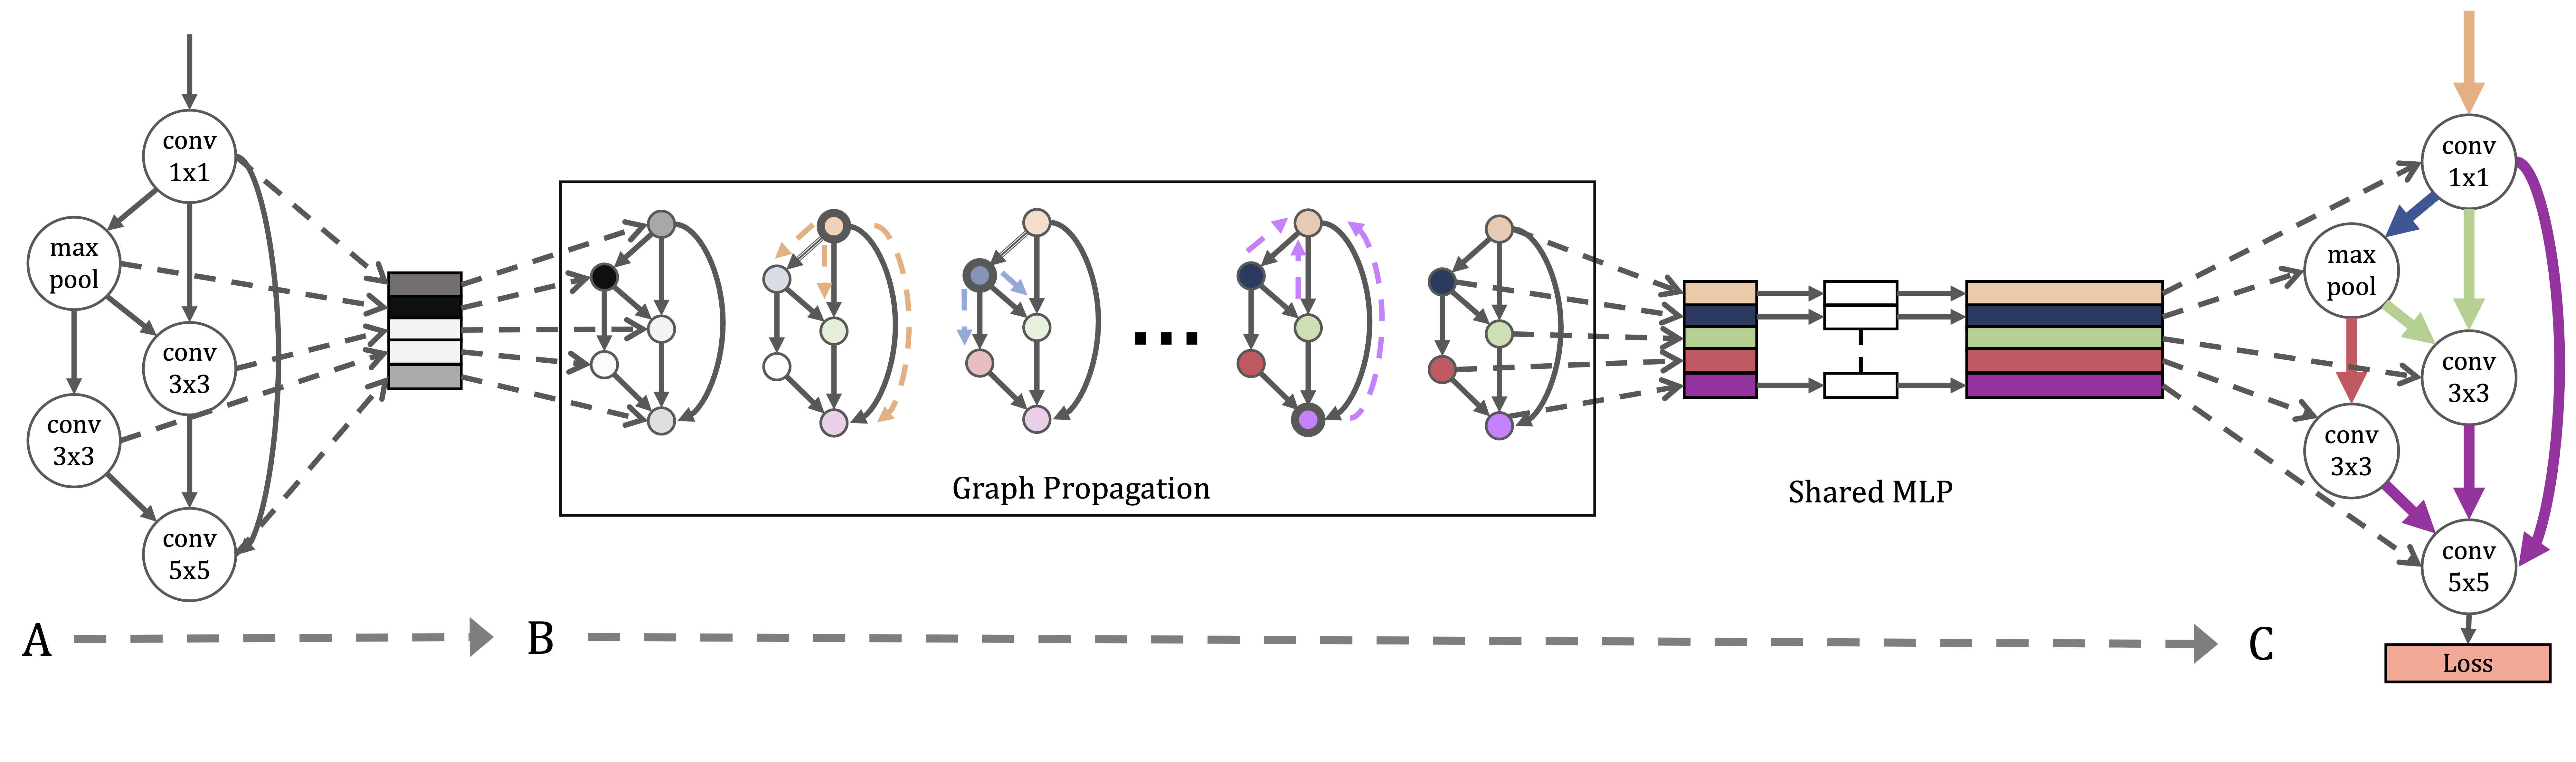
\includegraphics[width=6\linewidth]{figures/main3.png}
\else
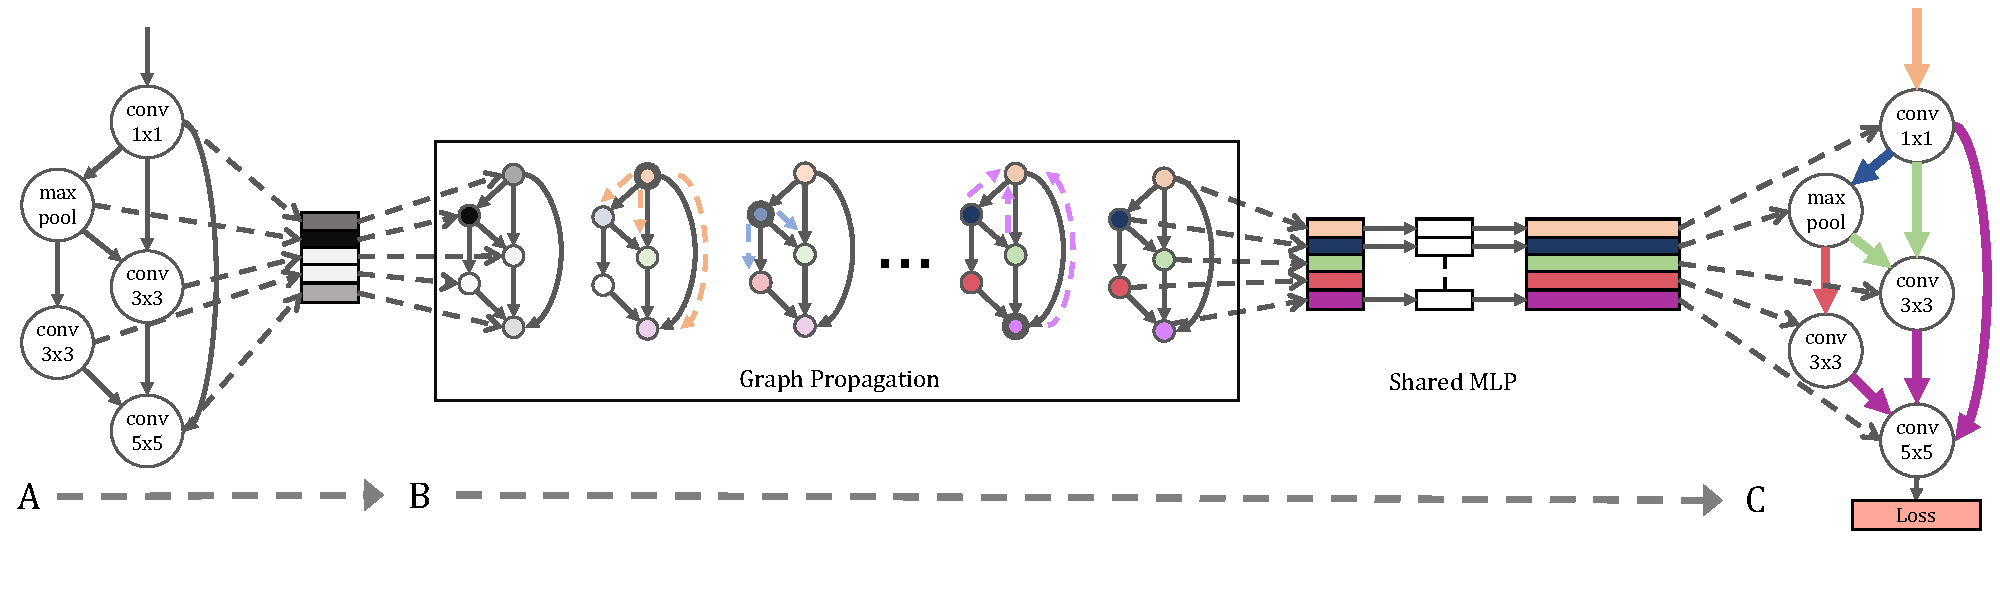
\includegraphics[width=\linewidth]{figures/main3.pdf}
\fi
\vspace{-1cm}
\caption{Our system diagram. \textbf{A}: A neural network architecture
is randomly sampled, forming a GHN. \textbf{B}: After graph propagation, each node in the GHN
generates its own weight parameters. \textbf{C}: The GHN is trained to minimize the training loss of
the sampled network with the generated weights. Random networks are ranked according to their
performance using GHN generated weights. }
\label{fig:main}
\vspace{-0.3cm}
\end{figure}

\subsection{Graphical Representation}
We represent a given architecture as a directed acyclic graph $\gA = (\gV, \gE)$, where each node $v
\in \gV$  has an associated computational operator $f_v$ parametrized by $w_v$, which produces an
output activation tensor $x_v$. Edges $e_{u \mapsto v} = (u, v) \in \gE$ represent the flow of
activation tensors from node $u$ to node $v$. $x_v$ is computed by applying its associated
computational operator on each of its inputs and taking summation as follows
\begin{equation}
\label{eq:compute_node}
x_v = \sum_{e_{u \mapsto v} \in \gE} f_v(x_u; w_v), \ \ \forall v \in \gV.
\end{equation}

\subsection{Graph Hypernetwork}
Our proposed Graph Hypernetwork is defined as a composition of a GNN and a hypernetwork. First,
given an input architecture, we used the graphical representation discussed above to form a graph
$\gA$. A parallel GNN $G_\gA$ is then constructed to be \textit{homomorphic} to $\gA$ with the exact
same topology. Node embeddings are initialized to one-hot vectors representing the node's
computational operator. After graph message-passing steps, a hypernet uses the node embeddings to
generate each node's associated parameters. Let $\vh_v^{(T)}$ be the embedding of node $v$ after $T$
steps of GNN propagation, and let $H \left(\cdot; \vvphi\right)$ be a hypernetwork parametrized by
$\vvphi$, the generated parameters $\tilde{\vw}_v$ are:
\begin{equation}
\tilde{\vw}_v = H \left(\vh_v^{(T)}; \vvphi\right).
\end{equation}
For simplicity, we implement $H$ with a multilayer perceptron (MLP). It is important to note that
$H$ is shared across all nodes, which can be viewed as an output prediction branch in each node of
the GNN. 
Thus the final set of generated weights of the entire architecture $\tilde{\vw}$ is found by applying $H$ on all the nodes and their respective embeddings which are computed by $G_\gA$:
\begin{align}
\tilde{\vw}=\left\{\tilde{\vw}_v | \ v \in \gV  \right\}
   &= \left\{H\left(\vh_v^{(T)}; \vvphi\right) \big| \ v \in \gV  \right\} \\
  &=  \left\{H\left(\vh; \vvphi\right) \big| \ \vh \in G_\gA^{(T)}\left(\left\{\vh_v^{(0)} \big| v \in \gV \right\}; \vphi\right)\right\} \\
  &= GHN\left(\gA; \vphi, \vvphi\right).
\end{align}

\subsection{Architectural Motifs and Stacked GNNs}
\label{section:graph_cells}

\iflatexml
\begin{figure}
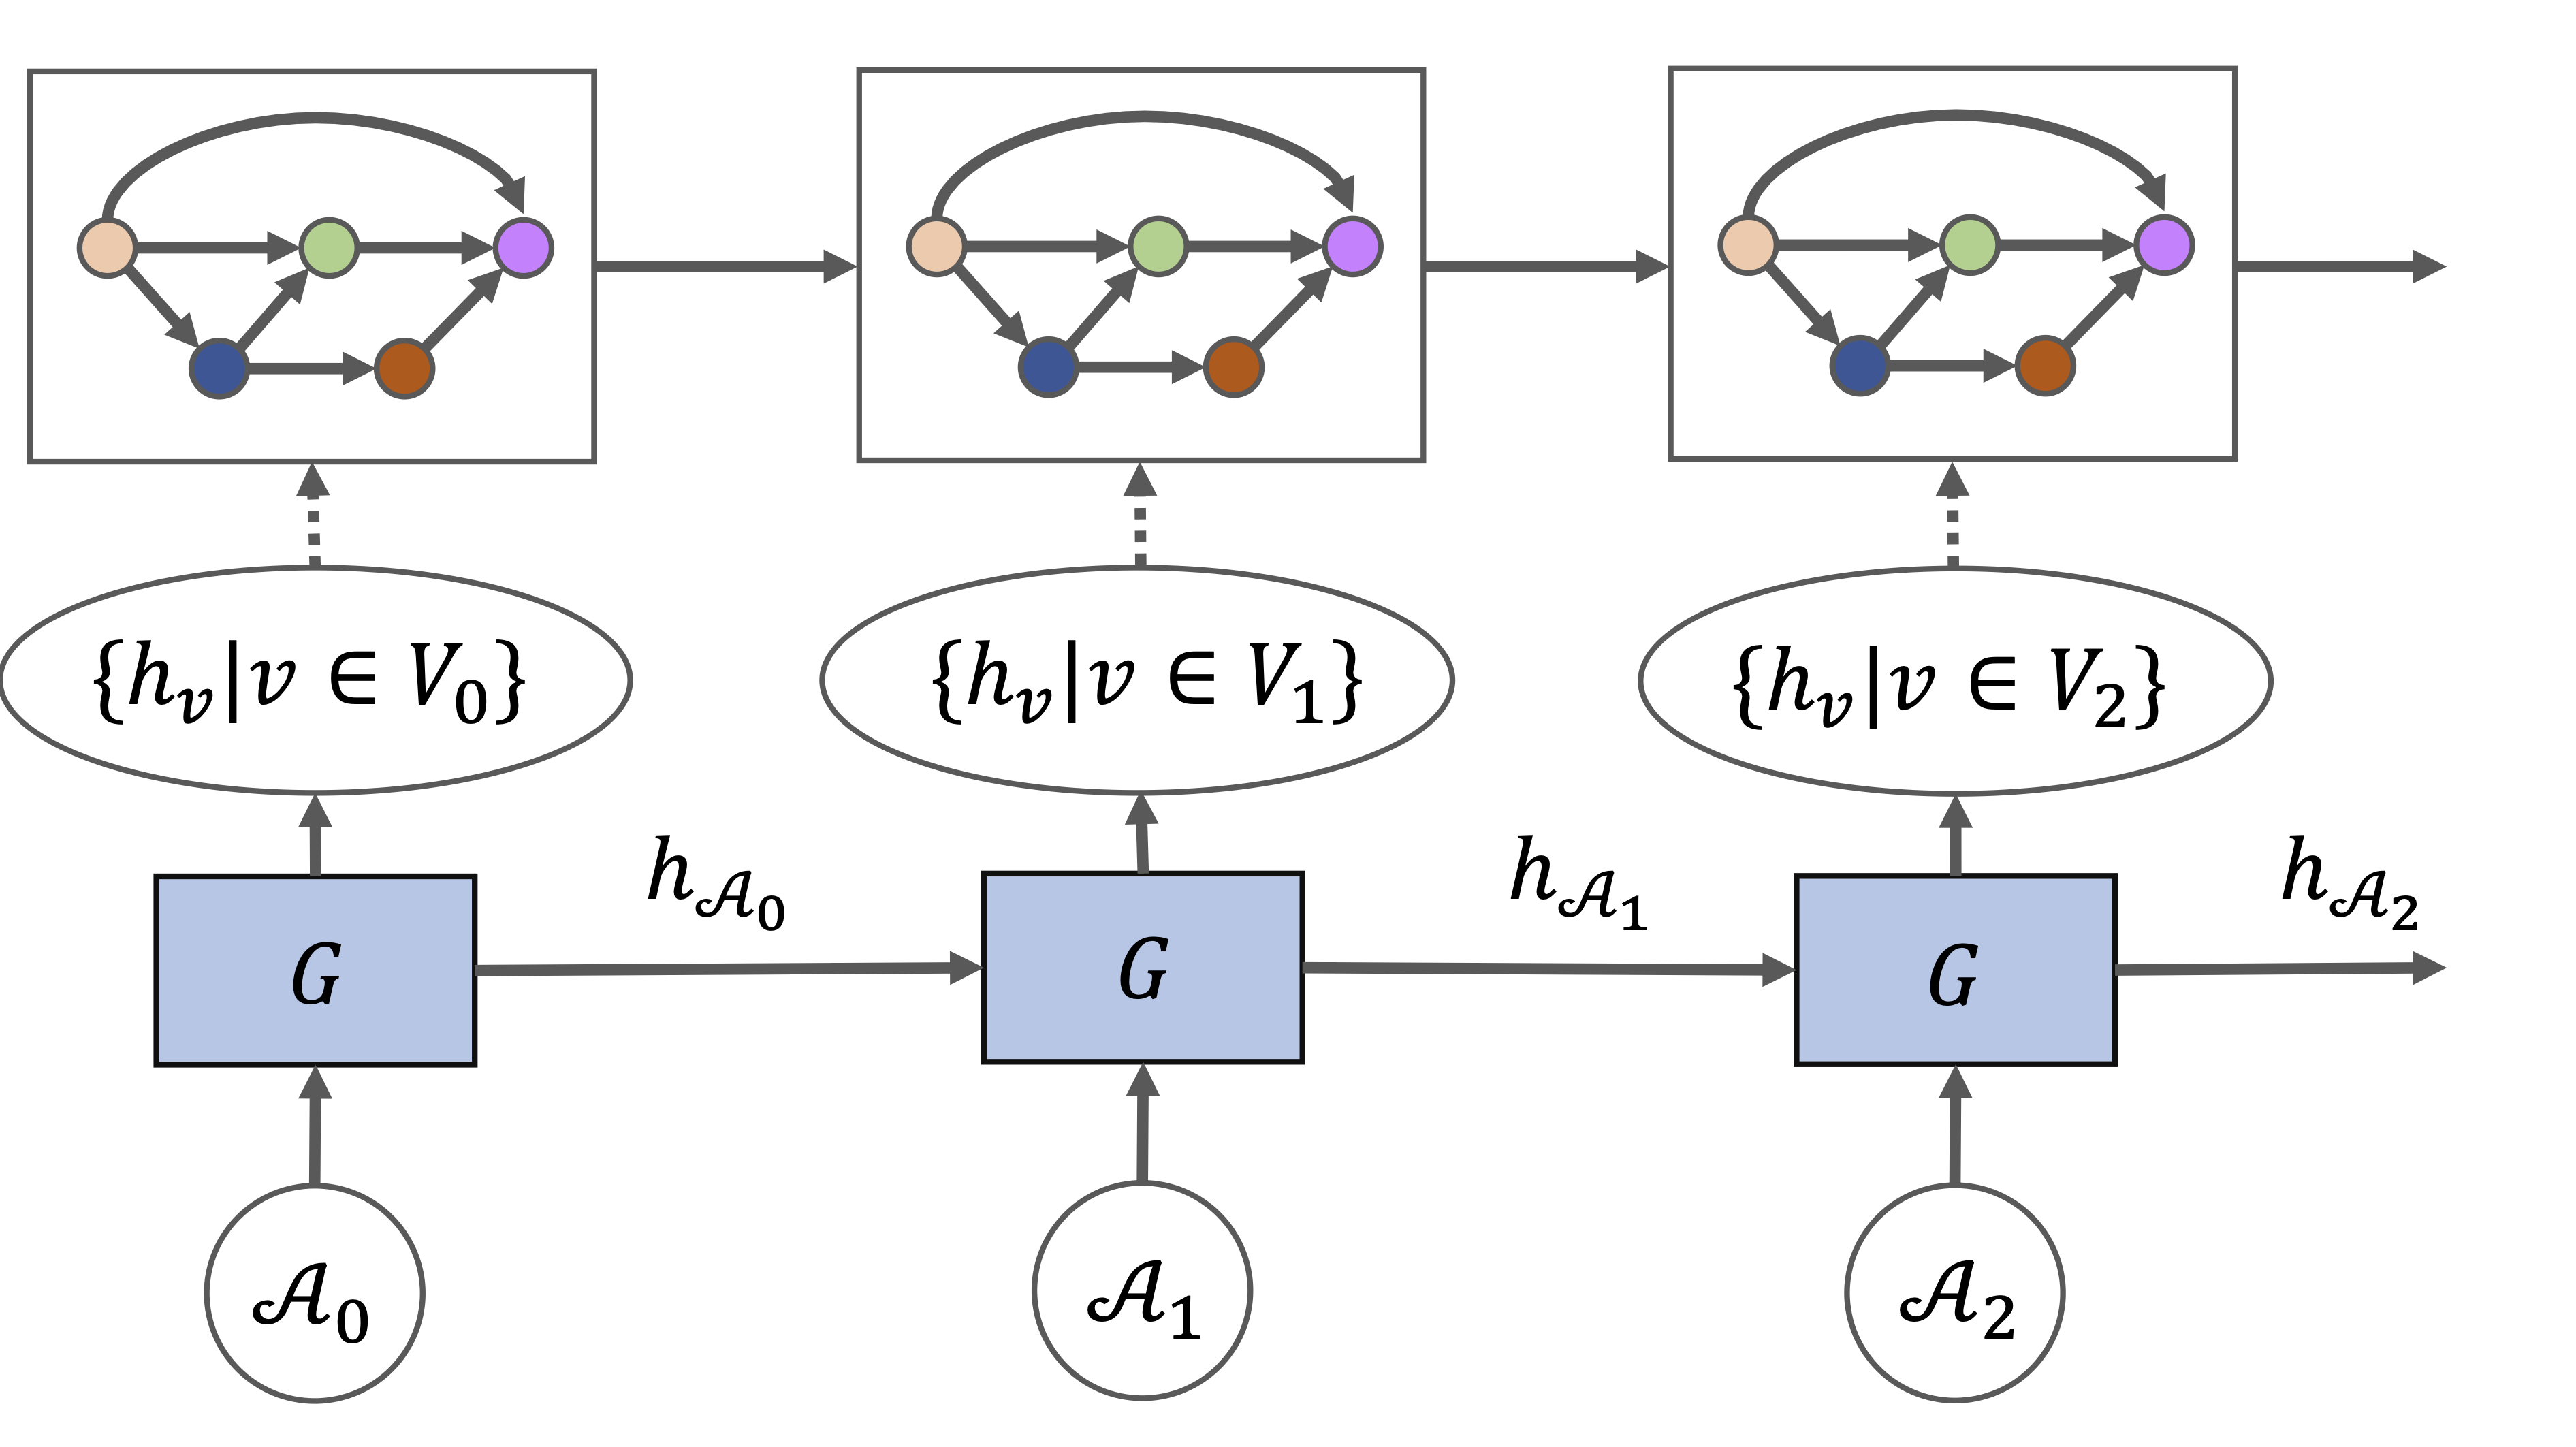
\includegraphics[width=4\linewidth]{figures/graph_cells.png}
\caption{Stacked GHN along the depth dimension.}
\label{fig:graph_cells}
\end{figure}
\else
\begin{wrapfigure}[]{r}{0.33\textwidth}
\vspace*{-0.5cm}
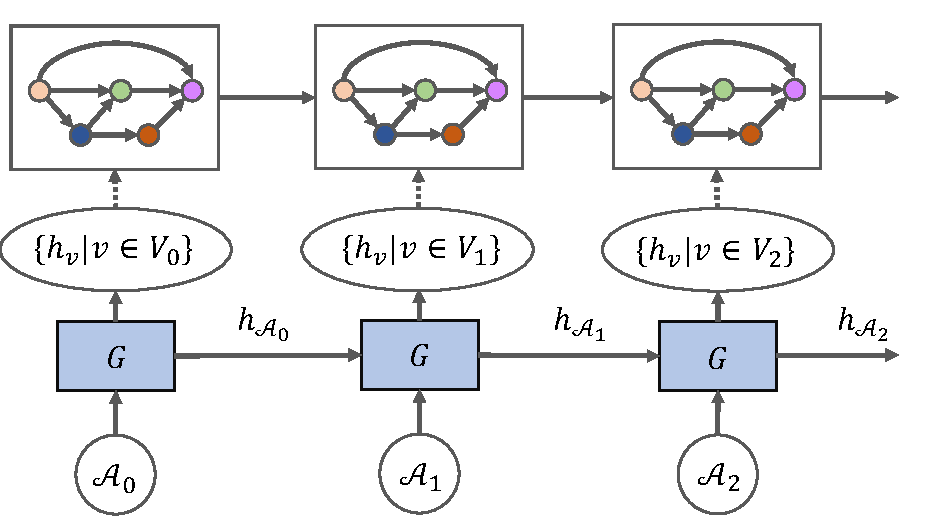
\includegraphics[width=\linewidth]{figures/graph_cells.pdf}
\caption{Stacked GHN along the depth dimension.}
\label{fig:graph_cells}
\end{wrapfigure}
\fi
The computation graph of some popular CNN architectures often spans over hundreds of nodes
\citep{he2016deep,huang2017densely}, which makes the search problem scale poorly. Repeated
architecture motifs are originally exploited in those architectures where the computation of each
computation block at different resolutions is the same, e.g. ResNet \citep{he2016resnet}. Recently,
the use of architectural motifs also became popular in the context of neural architecture search,
e.g. \citep{zoph2017learning, pham2018efficient}, where a small graph module with a fewer number of
computation nodes is searched, and the final architecture is formed by repeatedly stacking the same
module. \cite{zoph2017learning} showed that this leads to stronger performance due to a reduced
search space; the module can also be transferred to larger datasets by adopting a different
repeating pattern.

Our proposed method scales naturally with the design of repeated modules by stacking the same graph
hypernetwork along the depth dimension. Let $\gA$ be a graph composed of a chain of repeated modules
$\{\gA_i\}_{i=1}^N$. A graph level embedding $\vh_{\gA_i}$ is computed by taking an average over all
node embeddings after a full propagation of the current module, and passed onwards to the input node
of the next module as a message before graph propagation continues to the next module.
\begin{align}
\vh_{\gA_0} &= 0,\\
\vh_{\gA_i} &= \frac{1}{|\gV_i|}\sum_{v\in \gV_i} \left\{\vh_v^{(T)} | v \in \gV_i \right\} \label{eq:agg}\\
            &= \frac{1}{|\gV_i|}\sum G_{\gA_i}^{(T)}\left(\left\{\vh_v^{(0)} | v \in \gV_i \right\}, \vh_{\gA_{i-1}}; \vphi\right) \ \ \forall i > 0 \label{eq:next_cell}
\end{align}
Note that $G_{\gA_i}$ share parameters for all $\gA_i$.  Please see Figure~\ref{fig:graph_cells} for an overview.

\subsection{Forward-backward GNN message passing}
\label{sec:prop_scheme}
Standard GNNs employ the \textit{synchronous propagation scheme} \citep{li2015gated}, where the node
embeddings of all nodes are updated simultaneously at every step (see Equation~\ref{eq:gnn_prop}).
Recently, \cite{liao2018graph} found that such propagation scheme is inefficient in passing
long-range messages and suffers from the vanishing gradient problem as do regular RNNs. To mitigate
these shortcomings they proposed \textit{asynchronous propagation} using graph partitions. In our
application domain, deep neural architectures are chain-like graphs with a long diameter; This can
make synchronous message passing difficult. Inspired by the backpropagation algorithm, we propose
another variant of asynchronous propagation scheme, which we called \textit{forward-backward}
propagation, that directly mimics the order of node execution in a backpropagation algorithm.
Specifically, let $s$ be a topological sort of the nodes in the computation graph in a forward pass,
\begin{equation}
\label{eq:gnn_prop2}
\vh_v^{(t+1)} = 
\begin{cases}
U \left(\vh_v^{(t)}, \vm_v^{(t)} \right) \ \ & \text{if } s(t) = v \text{ and } 1 \le t \le |\gV|\\
  \ \ & \text{or if } s(2|\gV| - t) = v \text{ and } |\gV| + 1 \le t < 2|\gV|,\\
\vh_v^{(t)} \ \ & \text{otherwise}.
\end{cases}
\end{equation}
The total number of propagation steps $T$ for a full forward-backward pass will then become $2|\gV|-1$. Under the synchronous scheme,  propagating information across a graph with diameter $|\gV|$ would require $O(|\gV|^2)$ messages. This is reduced to $O(|\gV|)$ under the forward-backward scheme.

\subsection{Learning}
Learning a graph hypernetwork is straightforward since $\tilde{\vw}$ are directly generated by a
differentiable network. We compute gradients of the graph hypernetwork parameters $\vphi, \vvphi$
using the chain rule:
\begin{equation}
\nabla_{\vphi, \vvphi}{\gL_{train}(\tilde{\vw})} = \nabla_{\tilde{\vw}}{
\gL_{train}(\tilde{\vw})} \cdot \nabla_{\vphi, \vvphi}{\tilde{\vw}}
\end{equation}
The first term is the gradients of standard network parameters, the second term is decomposed as\begin{align}
 \nabla_\vphi{\tilde{\vw}} &= \left\{ \nabla_\vh H( \vh; \vvphi) \cdot \nabla_\vphi \vh \ \big| \ \vh \in G^{(T)} \left( \{\vh_v^{(0)}\}, \gA, \vphi \right) \right\}, \label{eq:gnn_grad}  \\ 
 \nabla_\vvphi{\tilde{\vw}} &= \left\{ \nabla_\vvphi H( \vh_v^{(T)}; \vvphi) \ \big| \ v \in \gV \right\} \label{eq:hypernet_grad}
\end{align}
where (Eq. \ref{eq:gnn_grad}) is the contribution from GNN module $G$ and (Eq.
\ref{eq:hypernet_grad}) is the contribution from the hypernet module $H$. Both $G$ and $H$ are
jointly learned throughout training.
% !TEX root = ../arxiv.tex
\savespacebeforesection
\section{Related Work}
\savespacebeforesection
\paragraph{Few-shot learning:}
Few-shot learning (FSL)~\citep{fei2006one,lake2011oneshot,matchingnet} entails
learning new tasks with only a few examples. With an abundance of training
data, FSL is closely related to the general meta-learning or learning to learn
paradigm~\citep {Thrun1998}, as a few-shot learning algorithm can be developed
on training tasks and run on novel tasks at test time. In standard few-shot
classification, each image only has a single unambiguous class label, whereas
in our few-shot attribute learning, the target attributes can vary depending on
how the support set is presented. We show in this paper that this is a more
challenging problem as it requires the model to be more flexible and
generalizable. In early benchmarks, a set of semantic classes was randomly
split into a training and test set. We hypothesize that this often leads to a
common set of attributes that span (most of) the training and test classes,
thus causing high transferability between these two sets, which allows simple
solutions based on feature re-use \citep{closerlook,anil} to work well. Later
benchmarks explicitly attempt to vary the separation between train and test
classes, based on varying the distances in the underlying WordNet classes
(\textit{tiered}-ImageNet \citep{fewshotssl}), or in different image domains
(Meta-Dataset \citep{triantafillou2019meta}). However, we argue that reasoning
about the underlying attributes directly offers a more systematic framework to
measure the relatedness and transferability between the train and test set. We
expect our analysis to open the door to such studies in the future. Few-shot
attribute learning is also related to multi-label few-shot
learning~\citep{alfassy2019laso,li2021compositional} and compositional few-shot learning~\citep{tokmakov2019learning}. These prior works
emphasize on the compositional aspect, whereas we propose models that address
the transferability of the learned representations.
Additionally,
\citet{xiang2019incremental} explored combining incremental few-shot learning
and attribute learning for pedestrian images.

\savespacebeforesection
\paragraph{Attribute learning:}
In the past, there have been a number of works that aim to predict attribute
information from raw
inputs~\citep{ferrari2007attribute,farhadi2009describe,farhadi2010attribute,wang2010discriminative}.
A related model is later proposed by \citet{koh2020concept} to achieve better
causal interpretability.% \citet{escorcia2015relationship} found that certain
% hidden units of a deep neural network predicts attributes very well. 
There have also been a number of datasets that have been collected with visual
attributes annotated
\citep{cub,zappos,celeba,patterson2016coco,pham2021attribute}. One key
difference between our work and these attribute learning approaches is that at
test time we aim to learn a classifier on novel attributes that are previously
not labeled in the training set, and this brings additional challenges of
transfer learning and learning with limited labeled data.

\savespacebeforesection
\paragraph{Zero-shot learning:} In zero-shot learning
(ZSL)~\citep{farhadi2009describe,labelembed,goodbadugly,attributezsl,ezzsl,evaluateoutput},
a model is asked to recognize classes not present in the training set,
supervised only by some auxiliary description~\citep{descriptionzsl} or
attribute values~\citep{farhadi2009describe} (see~\citet{wang2019survey} for a
survey). \citet{attributezsl} studied the \textit{direct attribute prediction}
method, similar to the Supervised Attribute baseline described in
Section~\ref{sec:baselines}. Compositional ZSL aims at learning
classes~\citep{czsl,taskdriven,taskaware,unseencomposition} defined by a novel
composition of labeled attributes and object classes. An important distinction
between ZSL and our few-shot attribute learning task is that ZSL uses the same
set of attributes for both training and testing; by contrast, our task asks the
model to learn attributes for which there are no labels during training, and
they may not be relevant to any of the training attributes or episodes. We
summarize the relationships between ZSL, FSL and our task in
Table~\ref{tab:benchmarkdiff}.

% \savespacebeforesection
% \paragraph{Context dependent similarity:} Unlike standard few-shot learning, in
% our learning episodes, the context information is essential for discovering the
% relevant attribute shared among the set of positive examples. The idea of
% context dependent similarity of features explored in the present work takes one
% step towards a more human-like decision maker. As an example provided by
% \citet{tversky1977features}, Cuba is similar to Jamaica in terms of geographic
% proximity, but similar to (Soviet) Russia when speaking of political
% viewpoints. Conditional similarity networks~\citep{condsimnet} proposed
% learning a feature mask for different pre-defined contexts such as colors or
% styles, using the triplet objective~\citep{finegrainsim}. Similarly,
% \citet{contextvissim} proposed to learn a different linear matrix for each
% context. In this paper, we study learning \textit{novel} contextual
% similarities in the form of attributes using only a few training examples.

\savespacebeforesection
\paragraph{Generalization to novel tasks:}
\looseness=-1 
One key component of our work is an attempt to understand the generalization
behavior of learning novel concepts at test time. Relevant theoretical studies
consider novel task generalization, casting it in a transfer learning and
learning to learn
framework~\citep{baxter2000model,ben2008notion,ben2010theory,pentina2014,amit2018meta,lucas2020lb}.
A common theme in these studies is in characterizing task relatedness, and the
role that it plays in generalization to novel tasks.
\citet{arnold2021embedding} studied task clustering for few-shot learning in
the embedding space and found class splits that are of different difficulty
levels. \citet{sariyildiz2021} use the WordNet hierarchy to compute semantic
distances. In our paper, we instead split the data in the attribute space, and
if we assume that semantic classes are combinations of attributes, then a
disjoint attribute split will imply further semantic distances.  In our work,
we investigate the role of task relatedness empirically by investigating
generalization performance under different splits of the attribute space.
% !TEX root = ../main.tex
\section{Experiments}
\vspace{-0.1in}
In this section, we show experimental results for our online contextualized few-shot learning
paradigm, using \ourchar{} and \ourroom{} (see Sec.~\ref{sec:benchmark}) to evaluate our model, CPM,
and other state-of-the-art methods. For Omniglot, we apply an 8$\times$8 CutOut~\citep{cutout} to
each image to make the task more challenging. 
% Details about the split information can be found in
% Appendix~\ref{app:data}.

\vspace{-0.1in} \paragraph{Implementation details:} For \ourchar{}, we use the common
4-layer CNN for few-shot learning with 64 channels in each layer. For \ourimg{}, we also use ResNet-12 
with input resolution 84$\times$84~\citep{tadam}. For the \ourroom{}, we resize the input to 
120$\times$160 and use ResNet-12. To represent
the feature of the input image with an attention mask, we concatenate the global average pooled
feature with the attention ROI feature, resulting in a 512d feature vector. For the contextual RNN,
in both experiments we used an LSTM~\citep{lstm} with a 256d hidden state. The best CPM model is
equipped using GAU and cosine similarity for querying prototypes. Logits based on cosine similarity
are multiplied with a learned scalar initialized at 10.0~\citep{tadam}. We include additional
training details in Appendix~\ref{app:exp}.

\vspace{-0.1in}
\paragraph{Evaluation metrics:}
In order to compute a single number that characterizes the learning ability over sequences, we
propose to use \textit{average precision} (AP) to evaluate
both with respect to old versus new and the
specific class predictions.
Concretely, all predictions are sorted by their old vs. new scores, and we compute AP using the area
under the precision-recall curve. A true positive is defined as the correct prediction of a
multi-class classification among known classes. We also compute the ``$N$-shot'' accuracy; i.e., the
average accuracy after seeing the label $N$ times in the sequence. Note that these accuracy scores
only reflect the performance on {\it known} class predictions. All numbers are reported with an
average over 2,000 sequences and for $N$-shot accuracy standard error is also included.
Further explanation of these metrics is in Appendix~\ref{sec:metrics}. 

\vspace{-0.1in}
\paragraph{Comparisons:}
To evaluate the merits of our proposed model, we implement classic few-shot learning and online
meta-learning methods. More implementation and training details of these baseline methods can be
found in Appendix~\ref{app:exp}.
% !TEX root = ../main.tex
\begin{figure}[t]
\vspace{-0.5in}
\centering
\iflatexml
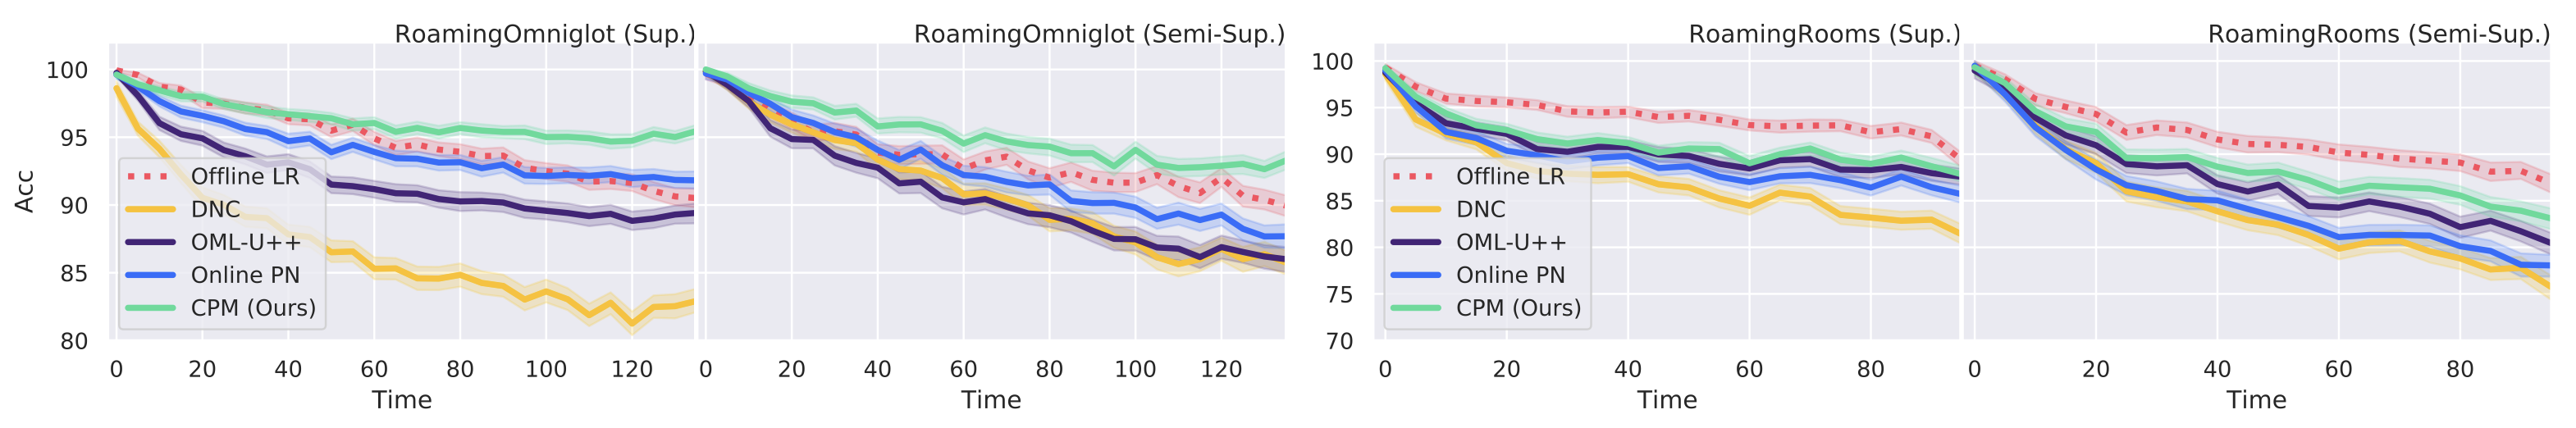
\includegraphics[width=6\linewidth]{figures/acctime_full.png}
\else
\setlength{\tabcolsep}{0pt}
\begin{tabular}{cccc}
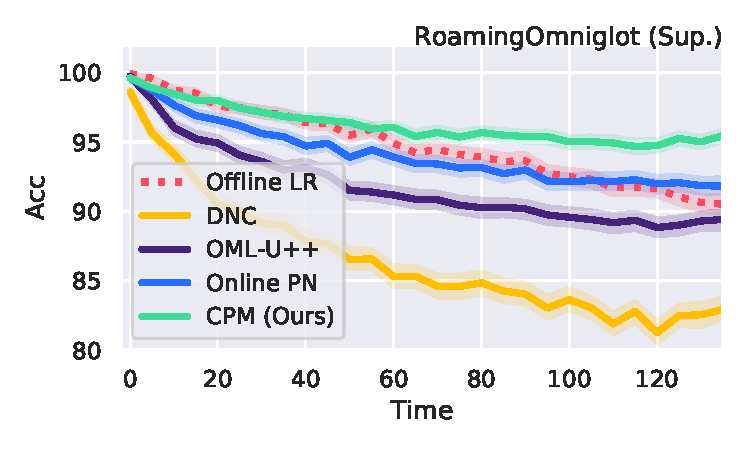
\includegraphics[height=2.4cm,trim={0.3cm 0cm 0.5cm 0},clip]{figures/omniglot-nossl-time.pdf}
&
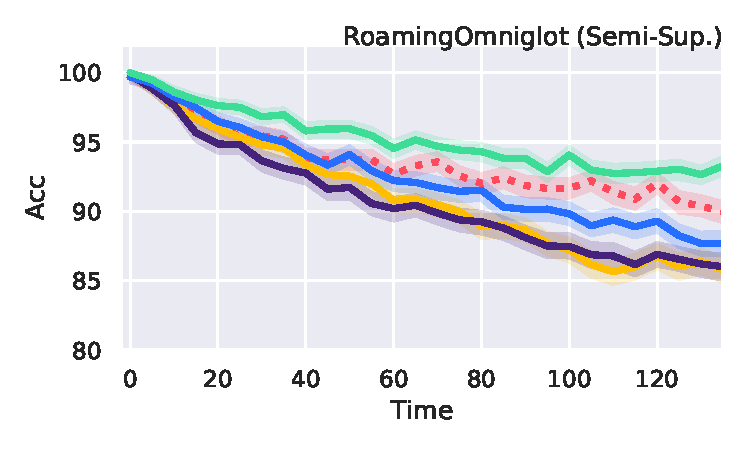
\includegraphics[height=2.4cm,trim={2cm 0cm 0cm 0},clip]{figures/omniglot-ssl-time.pdf}
&
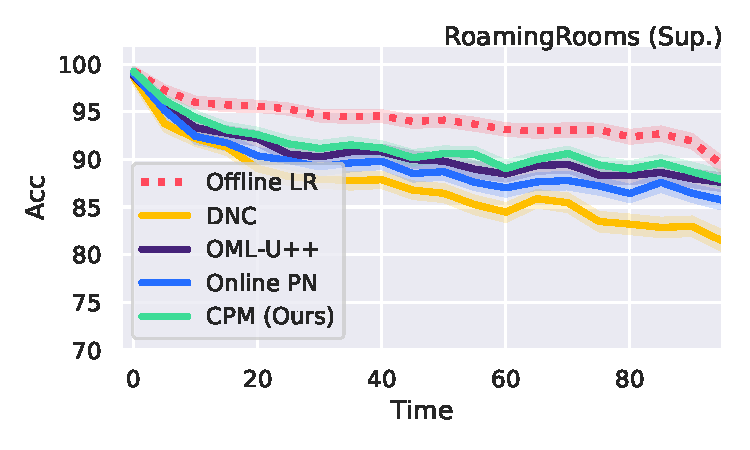
\includegraphics[height=2.4cm,trim={1cm 0cm 0.5cm 0},clip]{figures/matterport-nossl-time.pdf}
&
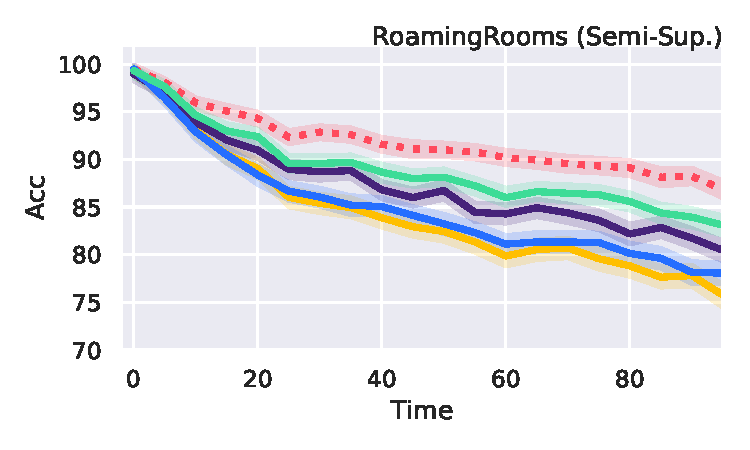
\includegraphics[height=2.4cm,trim={2cm 0cm 0cm 0},clip]{figures/matterport-ssl-time.pdf}
\\
\end{tabular}
\vspace{-0.25in}
\fi
\caption{\textbf{Few-shot classification accuracy over time.} \textbf{Left:} \ourchar{}.
\textbf{Right:} \ourroom{}. \textbf{Top:} Supervised. \textbf{Bottom:} Semi-supervised. An offline
logistic regression (Offline LR) baseline is also included, using pretrained ProtoNet features. It
is trained on all labeled examples except for the one at the current time step.}
\label{fig:acctimefull}
% \vspace{-0.25in}
\end{figure}

% !TEX root = ../main.tex
\begin{figure}[t]
\vspace{-0.1in}
\centering
\iflatexml
    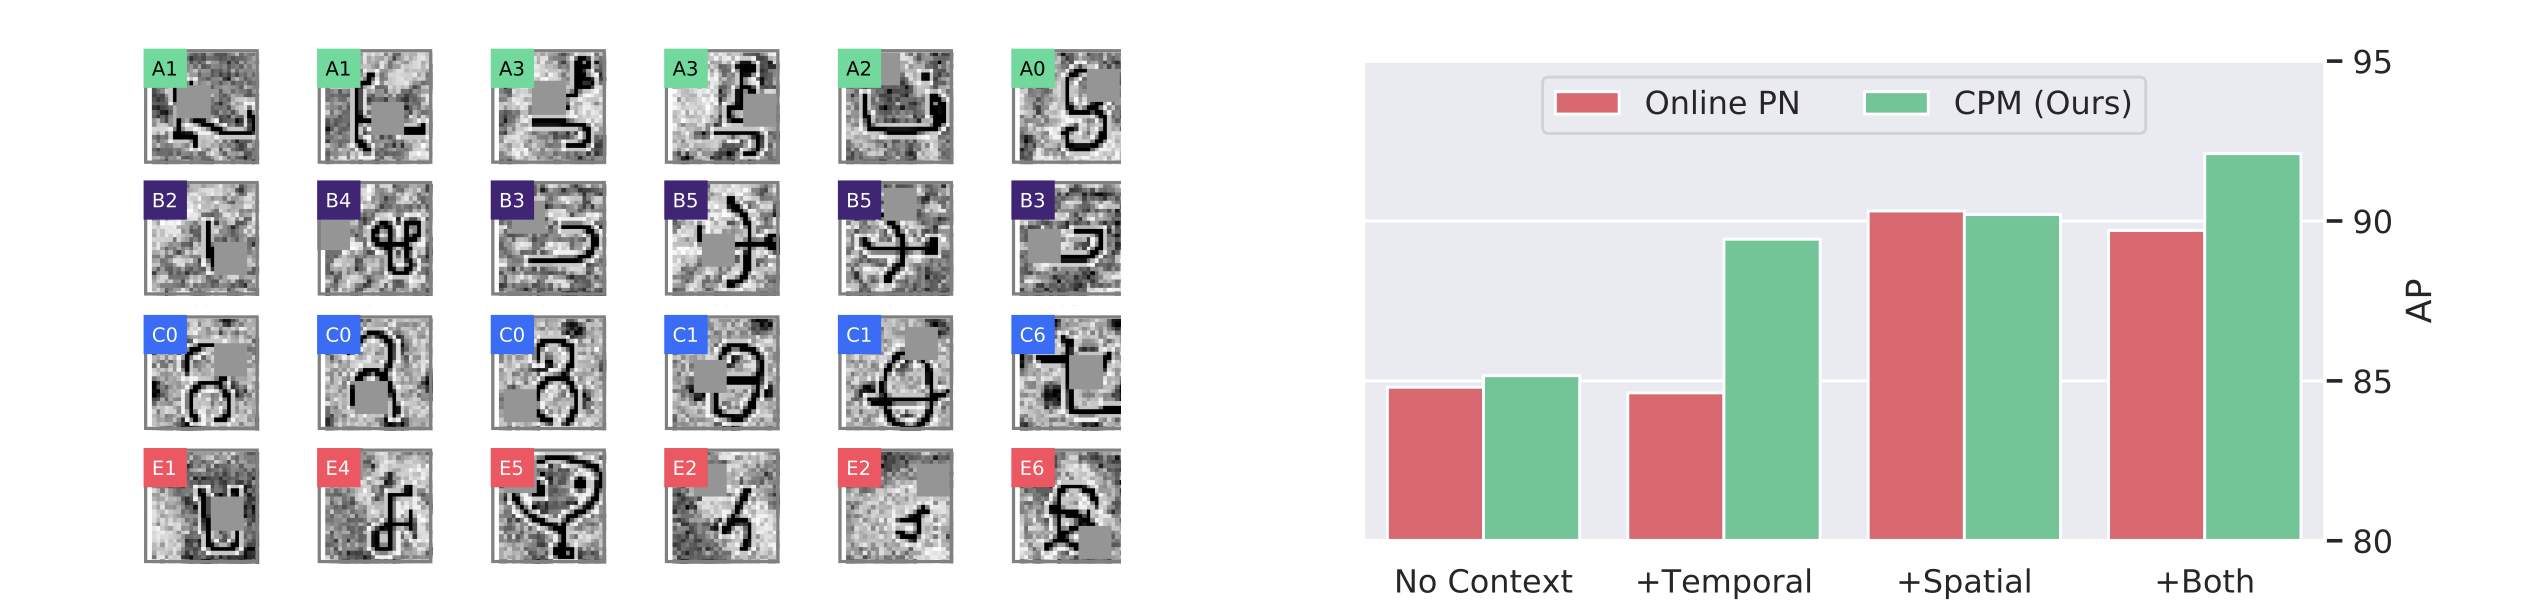
\includegraphics[width=6\linewidth]{figures/spatiotemporal_full.png}
\else
    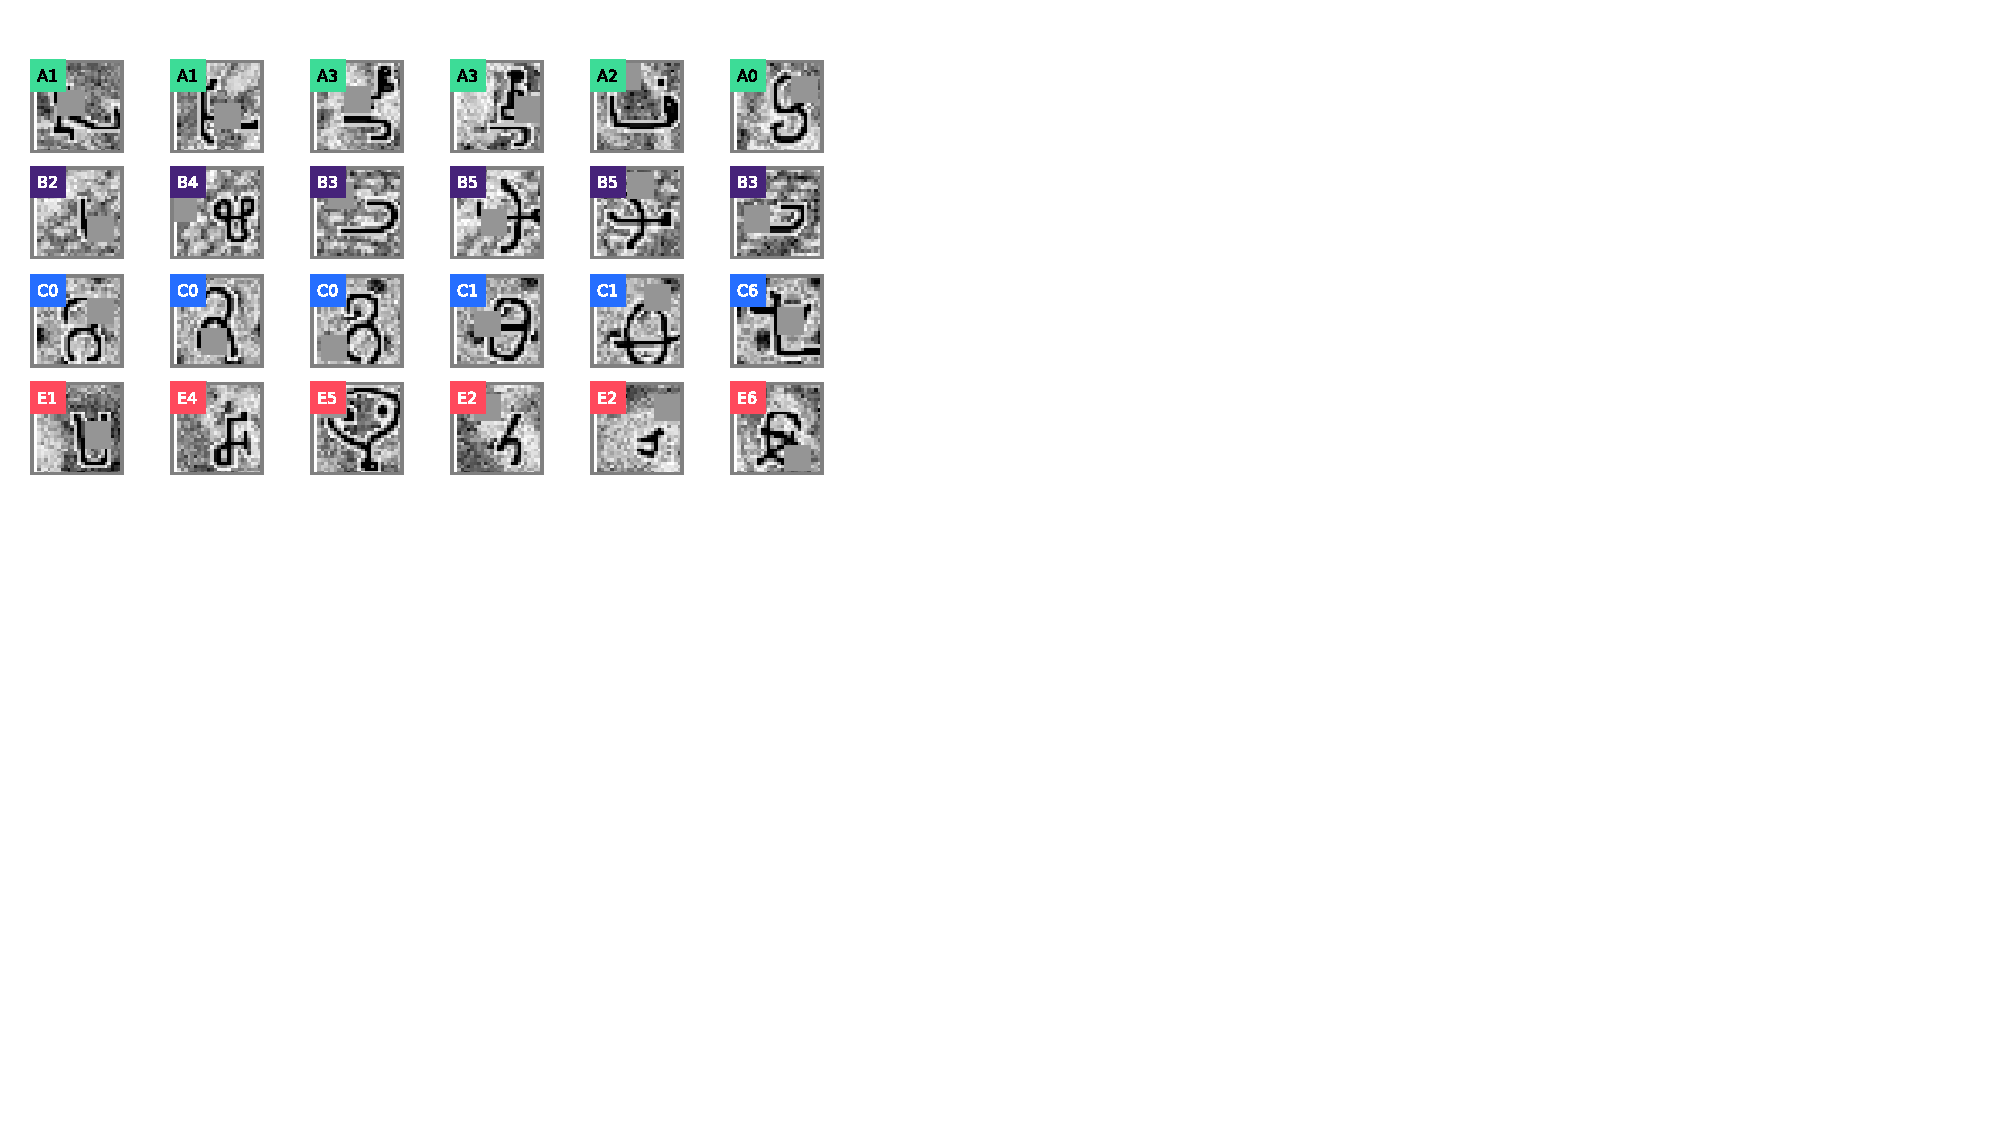
\includegraphics[height=2.8cm,trim={-2.25cm 10cm 20cm 0.5cm},clip]{figures/omniglot-texture.pdf}
    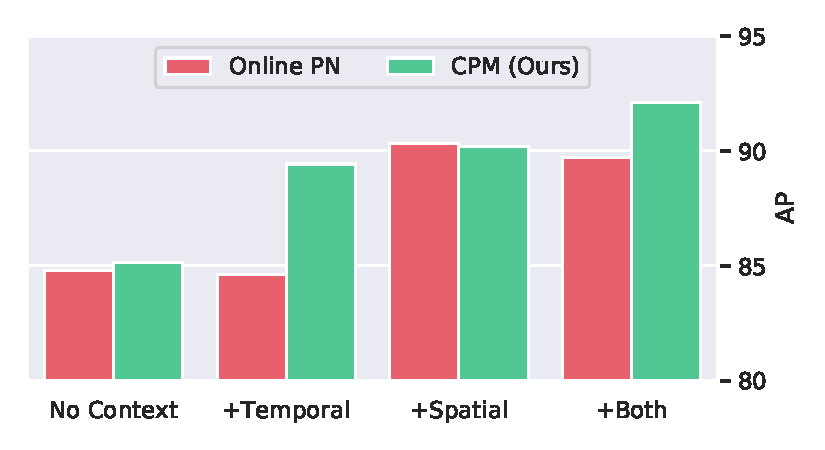
\includegraphics[height=2.8cm,trim={-2.25cm 0 0.5cm 0},clip]{figures/spatiotemporal.pdf}
\fi
\quad
\vspace{-0.2in}
\caption{\textbf{Effect of spatiotemporal context.} Spatiotemporal
context are added separately and together in \ourchar{}, by introducing texture background and
temporal correlation. \textbf{Left:} Stimuli used for spatial cue of the background environment.
\textbf{Right:} Our CPM model benefits from the presence of a temporal context
(``+Temporal'' and ``+Both'')} %, while Spatial context helps both CPM and online ProtoNet.}
\label{fig:spatiotemporal}
% \vspace{-0.1in}
\end{figure}

\vspace{-0.1in}
\iflatexml
\begin{itemize}
    \item \textbf{OML}~\citep{oml}: This is an online version of MAML~\citep{maml}. It performs one
    gradient descent step for each labeled input image, and slow weights are learned via
    backpropagation through time. On top of OML, we added an unknown predictor $\hat{u}_t = 1 -
    \max_k \hat{y}_{t,k}$ \footnote{We tried a few other ways and this is found to be the
    best.} (\textbf{OML-U}). We also found that using cosine classifier without the last layer ReLU
    is usually better than using the original dot-product classifier, and this improvement is denoted
    as \textbf{OML-U++}.
    \item \textbf{LSTM}~\citep{lstm} \& \textbf{DNC}~\citep{dnc}: We include RNN methods for
    comparison as well. Differentiable neural computer (DNC) is an improved version of memory
    augmented neural network (MANN)~\citep{mann}.
    \item \textbf{Online MatchingNet (\OnlineMatchingNet{})}~\citep{matchingnet}, 
    \textbf{IMP (\OnlineIMP{})}~\citep{imp} \&
    \textbf{ProtoNet (\OnlineProtoNet{})}~\citep{protonet}: We used\ the same negative Euclidean distance as the
    similarity function for these three metric learning based approaches.  In particular,
    MatchingNet stores all examples and performs nearest neighbor matching, which can be memory
    inefficient. Note that Online ProtoNet is a variant of our method without the contextual RNN.
\end{itemize}
\else
\begin{itemize}[leftmargin=*]
    \item \textbf{OML}~\citep{oml}: This is an online version of MAML~\citep{maml}. It performs one
    gradient descent step for each labeled input image, and slow weights are learned via
    backpropagation through time. On top of OML, we added an unknown predictor $\hat{u}_t = 1 -
    \max_k \hat{y}_{t,k}$ \footnote{We tried a few other ways and this is found to be the
    best.} (\textbf{OML-U}). We also found that using cosine classifier without the last layer ReLU
    is usually better than using the original dot-product classifier, and this improvement is denoted
    as \textbf{OML-U++}.
    \item \textbf{LSTM}~\citep{lstm} \& \textbf{DNC}~\citep{dnc}: We include RNN methods for
    comparison as well. Differentiable neural computer (DNC) is an improved version of memory
    augmented neural network (MANN)~\citep{mann}.
    \item \textbf{Online MatchingNet (\OnlineMatchingNet{})}~\citep{matchingnet}, 
    \textbf{IMP (\OnlineIMP{})}~\citep{imp} \&
    \textbf{ProtoNet (\OnlineProtoNet{})}~\citep{protonet}: We used\ the same negative Euclidean distance as the
    similarity function for these three metric learning based approaches.  In particular,
    MatchingNet stores all examples and performs nearest neighbor matching, which can be memory
    inefficient. Note that Online ProtoNet is a variant of our method without the contextual RNN.
\end{itemize}
\fi
\iflatexml
\begin{table}[t]
    \centering
    \begin{tabular}{ccccccc|cccccc}
    \toprule
    & \multicolumn{6}{c|}{\textbf{Supervised}} & \multicolumn{6}{c}{\textbf{Semi-Supervised}}\\
    Interval  &   1 - 2&      3 - 5&      6 - 10&     11 - 20&    21 - 50&    51 - 100&
                    1 - 2&      3 - 5&      6 - 10&     11 - 20&    21 - 50&    51 - 100\\
    OPN 1-Shot  &   88.8&       86.9&       85.2&       84.7&	    83.6&	    81.1&
                    90.1&       88.9&	    88.4&	    87.6&	    87.3&	    85.1\\
    CPM 1-Shot  &   \tb{96.1}&  \tb{94.0}&	\tb{93.0}&  \tb{91.6}&	\tb{88.2}&  \tb{84.6}&
                    \tb{95.9}&  \tb{93.8}&  \tb{92.8}&  \tb{91.8}&	\tb{89.4}&  \tb{85.7}\\
    OPN 3-Shot  &   97.2&	    97.1&	    96.6&	    96.7&	    \tb{96.5}&	95.3&
                    97.8&	    97.3&	    97.1&	    \tb{97.8}&	\tb{97.7}&  \tb{96.8}\\
    CPM 3-Shot  &   \tb{98.5}&	\tb{98.2}&	\tb{97.5}&	\tb{97.2}&      95.4&   \tb{95.5}&
                    \tb{98.7}&	\tb{97.5}&	\tb{97.5}&	    96.5&	    96.3&	    92.9\\
    \bottomrule
    \end{tabular}
    \caption{\textbf{Effect of forgetting over a time interval on \ourchar{}.} Average accuracy vs. the number of time steps since the model has last seen the label of a particular class.}
    \label{tab:forgetomniglot}
\end{table}
\else
\begin{table}[t]
\vspace{-0.5in}
    \centering
    \caption{\textbf{Effect of forgetting over a time interval on \ourchar{}.} Average accuracy vs. the number of time steps since the model has last seen the label of a particular class.}
    \vspace{0.1in}
    \resizebox{\textwidth}{!}{
    \begin{tabular}{ccccccc|cccccc}
    \toprule
    & \mc{6}{c}{\bf Supervised} & \mc{6}{c}{\bf Semi-Supervised}\\
    Interval  &   1 - 2&      3 - 5&      6 - 10&     11 - 20&    21 - 50&    51 - 100&
                    1 - 2&      3 - 5&      6 - 10&     11 - 20&    21 - 50&    51 - 100\\
    \midrule
    OPN 1-Shot  &   88.8&       86.9&       85.2&       84.7&	    83.6&	    81.1&
                    90.1&       88.9&	    88.4&	    87.6&	    87.3&	    85.1\\
    CPM 1-Shot  &   \bf{96.1}&  \bf{94.0}&	\bf{93.0}&	\bf{91.6}&	\bf{88.2}&  \bf{84.6}&
                    \bf{95.9}&  \bf{93.8}&  \bf{92.8}&	\bf{91.8}&	\bf{89.4}&	\bf{85.7}\\
    \midrule
    OPN 3-Shot  &   97.2&	    97.1&	    96.6&	    96.7&	    \bf{96.5}&	95.3&
                    97.8&	    97.3&	    97.1&	    \bf{97.8}&	\bf{97.7}&  \bf{96.8}\\
    CPM 3-Shot  &   \bf{98.5}&	\bf{98.2}&	\bf{97.5}&	\bf{97.2}&      95.4&  \bf{95.5}&
                    \bf{98.7}&	\bf{97.5}&	\bf{97.5}&	    96.5&	    96.3&	    92.9\\
    \bottomrule
    \end{tabular}}
    \label{tab:forgetomniglot}
\end{table}
\fi

% !TEX root = ../main.tex
\newcommand{\bgstar}{\beta_t^*, \gamma_t^*}
\newcommand{\bgw}{\beta_t^w$, $\gamma_t^w}
\newcommand{\hrnn}{\bh^{\text{RNN}}}


\iflatexml
    \begin{table}[t]
    \begin{center}
    \begin{tabular}{ccccccc}
    \toprule
    \tb{Method}                   & $\hrnn$ & $\bgstar$ & Metric $\bmm_t$ & GAU  & Val AP      \\
    \midrule                                                            
    \OnlineProtoNet{}             &         &           &                 &      & 91.22       \\
    No $\bh^{\text{RNN}}$         &         &  \yes     & \yes            &      & 92.52       \\
    $\bh^{\text{RNN}}$ only       & \yes    &           &                 &      & 93.48       \\
    No metric $\bmm_t$            & \yes    &  \yes     &                 &      & 93.61       \\
    No $\beta_t^*, \gamma_t^*$    & \yes    &           & \yes            &      & 93.98       \\
    $\bh_t = \bh_t^{\text{RNN}}$  & \yes    &  \yes     & \yes            &      & 93.70       \\
    CPM Avg. Euc                  & \yes    &  \yes     & \yes            &      & 94.08       \\
    CPM Avg. Cos                  & \yes    &  \yes     & \yes            &      & 94.57       \\
    CPM GAU Euc                   & \yes    &  \yes     & \yes            & \yes & 94.11       \\
    CPM GAU Cos                   & \yes    &  \yes     & \yes            & \yes & \tb{94.65}  \\
    \bottomrule
    \end{tabular}
    \end{center}
    \caption{Ablation of CPM architectural components on \ourchar{}}
    \label{tab:ablation} 
    \end{table}

    \begin{table}[t]
    \begin{center}
    \begin{tabular}{cccccccc}
    \toprule
    \tb{Method}         & RNN   & Prototype & $\bgw$ & GAU  & Val AP     \\
    \midrule                                                                                   
    \OnlineProtoNet{}   &       &           &        &      & 90.83      \\
    \OnlineProtoNet{}   &       &  \yes     &        &      & 89.10      \\
    \OnlineProtoNet{}   &       &  \yes     & \yes   &      & 91.22      \\
    CPM                 &       &           &        &      & 92.57      \\
    CPM                 &  \yes &           &        &      & 93.16      \\
    CPM                 &  \yes &  \yes     &        &      & 93.20      \\
    CPM                 &  \yes &  \yes     & \yes   &      & 94.08      \\
    CPM                 &  \yes &  \yes     & \yes   & \yes & \tb{94.65} \\
    \bottomrule
    \end{tabular}
    \end{center}
    \caption{Ablation of semi-supervised learning components on \ourchar{}}
    \label{tab:ablationssl}
    \end{table}
\else
    \begin{table}[t]
    \vspace{-0.1in}
    \begin{minipage}[t]{0.45\textwidth}
    \begin{small}
    \caption{Ablation of CPM architectural components on \ourchar{}}
    \begin{center}
    \label{tab:ablation}
    \resizebox{!}{1.4cm}{
    \begin{tabular}{ccccccc}
    \toprule
    \tb{Method}                   & $\hrnn$ & $\bgstar$ & Metric $\bmm_t$ & GAU  & Val AP      \\
    \midrule                                                            
    \OnlineProtoNet{}             &         &           &                 &      & 91.22       \\
    No $\bh^{\text{RNN}}$         &         &  \yes     & \yes            &      & 92.52       \\
    $\bh^{\text{RNN}}$ only       & \yes    &           &                 &      & 93.48       \\
    No metric $\bmm_t$            & \yes    &  \yes     &                 &      & 93.61       \\
    No $\beta_t^*, \gamma_t^*$    & \yes    &           & \yes            &      & 93.98       \\
    $\bh_t = \bh_t^{\text{RNN}}$  & \yes    &  \yes     & \yes            &      & 93.70       \\
    CPM Avg. Euc                  & \yes    &  \yes     & \yes            &      & 94.08       \\
    CPM Avg. Cos                  & \yes    &  \yes     & \yes            &      & 94.57       \\
    CPM GAU Euc                   & \yes    &  \yes     & \yes            & \yes & 94.11       \\
    CPM GAU Cos                   & \yes    &  \yes     & \yes            & \yes & \tb{94.65}  \\
    \bottomrule
    \end{tabular}
    }
    \end{center}
    \end{small}
    \end{minipage}
    \hfill
    \begin{minipage}[t]{0.45\textwidth}
    \caption{Ablation of semi-supervised learning components on \ourchar{}}
    \begin{small}
    \begin{center}
    \label{tab:ablationssl}
    \resizebox{!}{1.4cm}{
    \begin{tabular}{cccccccc}
    \toprule
    \tb{Method}         & RNN   & Prototype & $\bgw$ & GAU  & Val AP     \\
    \midrule                                                                                   
    \OnlineProtoNet{}   &       &           &        &      & 90.83      \\
    \OnlineProtoNet{}   &       &  \yes     &        &      & 89.10      \\
    \OnlineProtoNet{}   &       &  \yes     & \yes   &      & 91.22      \\
    CPM                 &       &           &        &      & 92.57      \\
    CPM                 &  \yes &           &        &      & 93.16      \\
    CPM                 &  \yes &  \yes     &        &      & 93.20      \\
    CPM                 &  \yes &  \yes     & \yes   &      & 94.08      \\
    CPM                 &  \yes &  \yes     & \yes   & \yes & \tb{94.65} \\
    \bottomrule
    \end{tabular}
    }
    \end{center}
    \end{small}
    \end{minipage}
    \vspace{-0.1in}
    \end{table}
 \fi


\vspace{-0.1in}
\paragraph{Main results:} Our main results are shown in Table~\ref{tab:omniglot}, 
\ref{tab:matterport} and \ref{tab:imagenet}, including both supervised and semi-supervised settings. Our approach achieves
the best performance on AP consistently across all settings. Online ProtoNet is a direct comparison
without our contextual RNN and it is clear that CPM is significantly better. Our method is slightly
worse than Online MatchingNet in terms of 3-shot accuracy on the \ourroom{} semisupervised
benchmark. This can be explained by the fact that MatchingNet stores all past seen examples, whereas
CPM only stores one prototype per class. Per timestep accuracy is plotted in
Figure~\ref{fig:acctimefull}, and the decaying accuracy is due to the increasing number of classes
over time. In \ourchar{}, CPM is able to closely match or even sometimes surpass the offline
classifier, which re-trains at each step and uses all images in a sequence except the current one. This is
reasonable as our model is able to leverage information from the current context.

\vspace{-0.1in}
\paragraph{Effect of spatiotemporal context:} To answer the question whether the gain in performance
is due to spatiotemporal reasoning, we conduct the following experiment comparing CPM with online
ProtoNet. We allow the CNN to have the ability to recognize the context in \ourchar{} by adding a
texture background image using the Kylberg texture dataset~\citep{uppsala} (see
Figure~\ref{fig:spatiotemporal} left). As a control, we can also destroy the temporal context by
shuffling all the images in a sequence. We train four different models on dataset controls with or
without the presence of spatial or temporal context, and results are shown in
Figure~\ref{fig:spatiotemporal}. First, both online ProtoNet and CPM benefit from the inclusion of a
spatial context. This is understandable as the CNN has the ability to learn spatial cues, which
re-confirms our  main hypothesis that successful inference of the current context is beneficial to
novel object recognition. Second, only our CPM model benefits from the presence of temporal context,
and it receives distinct gains from spatial and temporal contexts.

\vspace{-0.1in}
\paragraph{Effect of forgetting:} As the number of learned classes increases, we expect the average accuracy to drop. To further investigate this forgetting effect, we measure the average accuracy in terms of the number of time steps the model has last seen the label of a particular class. It is reported in Table~\ref{tab:forgetomniglot} and in Appendix~\ref{sec:additionalresults} Table~\ref{tab:forgetroom}, \ref{tab:forgetimagenet}, where we directly compare CPM and OPN to see the effect of temporal context.
CPM is significantly better than OPN on 1-shot within a short interval, which suggests that the contextual RNN 
makes the recall of the recent past much easier. On \ourimg{}, OPN eventually surpasses CPM on longer horizon, and this can be explained by the fact that OPN has more stable prototypes, whereas prototypes in CPM could potentially be affected by the fluctuation of the contextual RNN over a longer horizon.

\vspace{-0.1in}
\paragraph{Ablation studies:} We ablate each individual module we introduce. Results are shown in
Tables~\ref{tab:ablation} and~\ref{tab:ablationssl}. Table~\ref{tab:ablation} studies different ways
we use the RNN, including the context vector $\bh^{\text{RNN}}$, the predicted threshold parameters
$\beta_t^*,\gamma_t^*$, and the predicted metric scaling vector $\bmm_{t}$. Table~\ref{tab:ablationssl}
studies various ways to learn from unlabeled examples, where we separately disable the RNN update,
prototype update, and distinct write-threshold parameters $\beta^w_t, \gamma^w_t$ (vs. using
read-threshold parameters), which makes it robust to potential mistakes made in
semi-supervised learning. We verify that each component has a positive impact on the performance.

% !TEX root = ../main.tex
\vspace{-0.1in}
\section{Conclusion}
In this work, we propose an end-to-end learned, sparse visual attention
mechanism for self-driving, where the sparse attention mask gates the feature backbone
computation. As opposed to existing methods that focus on using attention for perception only,
our attention masks are directly optimized for motion planning, which enables our network to output
better planned trajectories while achieving more efficiency with higher sparsity. In future work,
the attention module can be extended to have recurrent feedbacks from the output layers
to better leverage temporal information.

% !TEX root = ../main.tex
\paragraph{Acknowledgement}
Supported by the Intelligence Advanced Research Projects Activity (IARPA) via Department of
Interior/Interior Business Center (DoI/IBC) contract number D16PC00003. The U.S. Government is
authorized to reproduce and distribute reprints for Governmental purposes notwithstanding any
copyright annotation thereon. Disclaimer: The views and conclusions contained herein are those of
the authors and should not be interpreted as necessarily representing the official policies or
endorsements, either expressed or implied, of IARPA, DoI/IBC, or the U.S. Government.


\bibliography{references}
\bibliographystyle{iclr2018_conference}

\newpage
\appendix
% !TEX root = ../main.tex
\section{Omniglot Dataset Details}
We used the following split details for experiments on Omniglot dataset. This is the same train/test split as \citep{vinyals2016matchingnet}, but we created our own validation split for selecting hyper-parameters. Models are trained on the train split only.

\textbf{Train Alphabets:}
Alphabet\_of\_the\_Magi,
Angelic,
Anglo-Saxon\_Futhorc,
Arcadian,
Asomtavruli\_(Georgian),
Atemayar\_Qelisayer,
Atlantean,
Aurek-Besh,
Avesta,
Balinese,
Blackfoot\_(Canadian\_Aboriginal\_Syllabics),
Braille,
Burmese\_(Myanmar),
Cyrillic,
Futurama,
Ge\_ez,
Glagolitic,
Grantha,
Greek,
Gujarati,
Gurmukhi (character 01-41),
Inuktitut\_(Canadian\_Aboriginal\_Syllabics),
Japanese\_(hiragana),
Japanese\_(katakana),
Korean,
Latin,
Malay\_(Jawi\_-\_Arabic),
N\_Ko,
Ojibwe\_(Canadian\_Aboriginal\_Syllabics),
Sanskrit,
Syriac\_(Estrangelo),
Tagalog,
Tifinagh

\textbf{Validation Alphabets:}
Armenian, 
Bengali, 
Early\_Aramaic, 
Hebrew, 
Mkhedruli\_(Geogian) 

\textbf{Test Alphabets:}
Gurmukhi (character 42-45),
Kannada,
Keble,
Malayalam,
Manipuri,
Mongolian,
Old\_Church\_Slavonic\_(Cyrillic),
Oriya,
Sylheti,
Syriac\_(Serto),
Tengwar,
Tibetan,
ULOG

\section{\textit{tiered}Imagenet Dataset Details}

Each high-level category in \textit{tiered}ImageNet contains between 10 and 30 ILSVRC-12 classes (17.8 on average). In the ImageNet hierarchy, some classes have multiple parent nodes. Therefore, classes belonging to more than one category were removed from the dataset to ensure separation between training and test categories. Test
categories were chosen to reflect various levels of separation between training
and test classes. Some test categories (such as ``working dog'') are fairly similar to training categories, whereas others (such as ``geological formation'')
are quite different. The list of categories is shown below and statistics of the dataset can be found in Table~\ref{tab:tiered_stats}. A visualization of the categories according to the ImageNet hierarchy is shown in Figure~\ref{fig:tiered_hierarchy}. The full list of classes per category will
also be made public, however for the sake of brevity we do not include it here.

\begin{table}[ht]
    \center
    \caption{Statistics of the \textit{tiered}ImageNet dataset.}
    \label{tab:tiered_stats}
    \begin{tabular}{l|cccc}
                   & Train   & Val & Test    & Total \\ \hline
        Categories & 20      & 6   & 8       & 34 \\
        Classes    & 351     & 97  & 160     & 608 \\
        Images     & 448,695 & 124,261   & 206,209 & 779,165 \\
    \end{tabular}
\end{table}

\textbf{Train Categories}:  
\texttt{n02087551} (hound, hound dog), 
\texttt{n02092468} (terrier),  
\texttt{n02120997} (feline, felid),  
\texttt{n02370806} (ungulate, hoofed mammal),
\texttt{n02469914} (primate),  
\texttt{n01726692} (snake, serpent, ophidian),  
\texttt{n01674216} (saurian),
\texttt{n01524359} (passerine, passeriform bird),  
\texttt{n01844917} (aquatic bird),  
\texttt{n04081844} (restraint, constraint),  
\texttt{n03574816} (instrument),  
\texttt{n03800933} (musical instrument, instrument),  
\texttt{n03125870} (craft),
\texttt{n04451818} (tool),  
\texttt{n03414162} (game equipment),
\texttt{n03278248} (electronic equipment),  
\texttt{n03419014} (garment), 
\texttt{n03297735} (establishment), 
\texttt{n02913152} (building, edifice),
\texttt{n04014297} (protective covering, protective cover, protection).

\textbf{Validation Categories}: 
\texttt{n02098550} (sporting dog, gun dog),
\texttt{n03257877} (durables, durable goods, consumer durables),
\texttt{n03405265} (furnishing),
\texttt{n03699975} (machine),  
\texttt{n03738472} (mechanism),
\texttt{n03791235} (motor vehicle, automotive vehicle), 


\textbf{Test Categories}: \texttt{n02103406} (working dog),  \texttt{n01473806} (aquatic vertebrate),
\texttt{n02159955} (insect), \texttt{n04531098} (vessel),
\texttt{n03839993} (obstruction, obstructor, obstructer, impediment, impedimenta),
\texttt{n09287968} (geological formation, formation), \texttt{n00020090} (substance),  \texttt{n15046900} (solid).


\iflatexml
\begin{figure}[ht]
    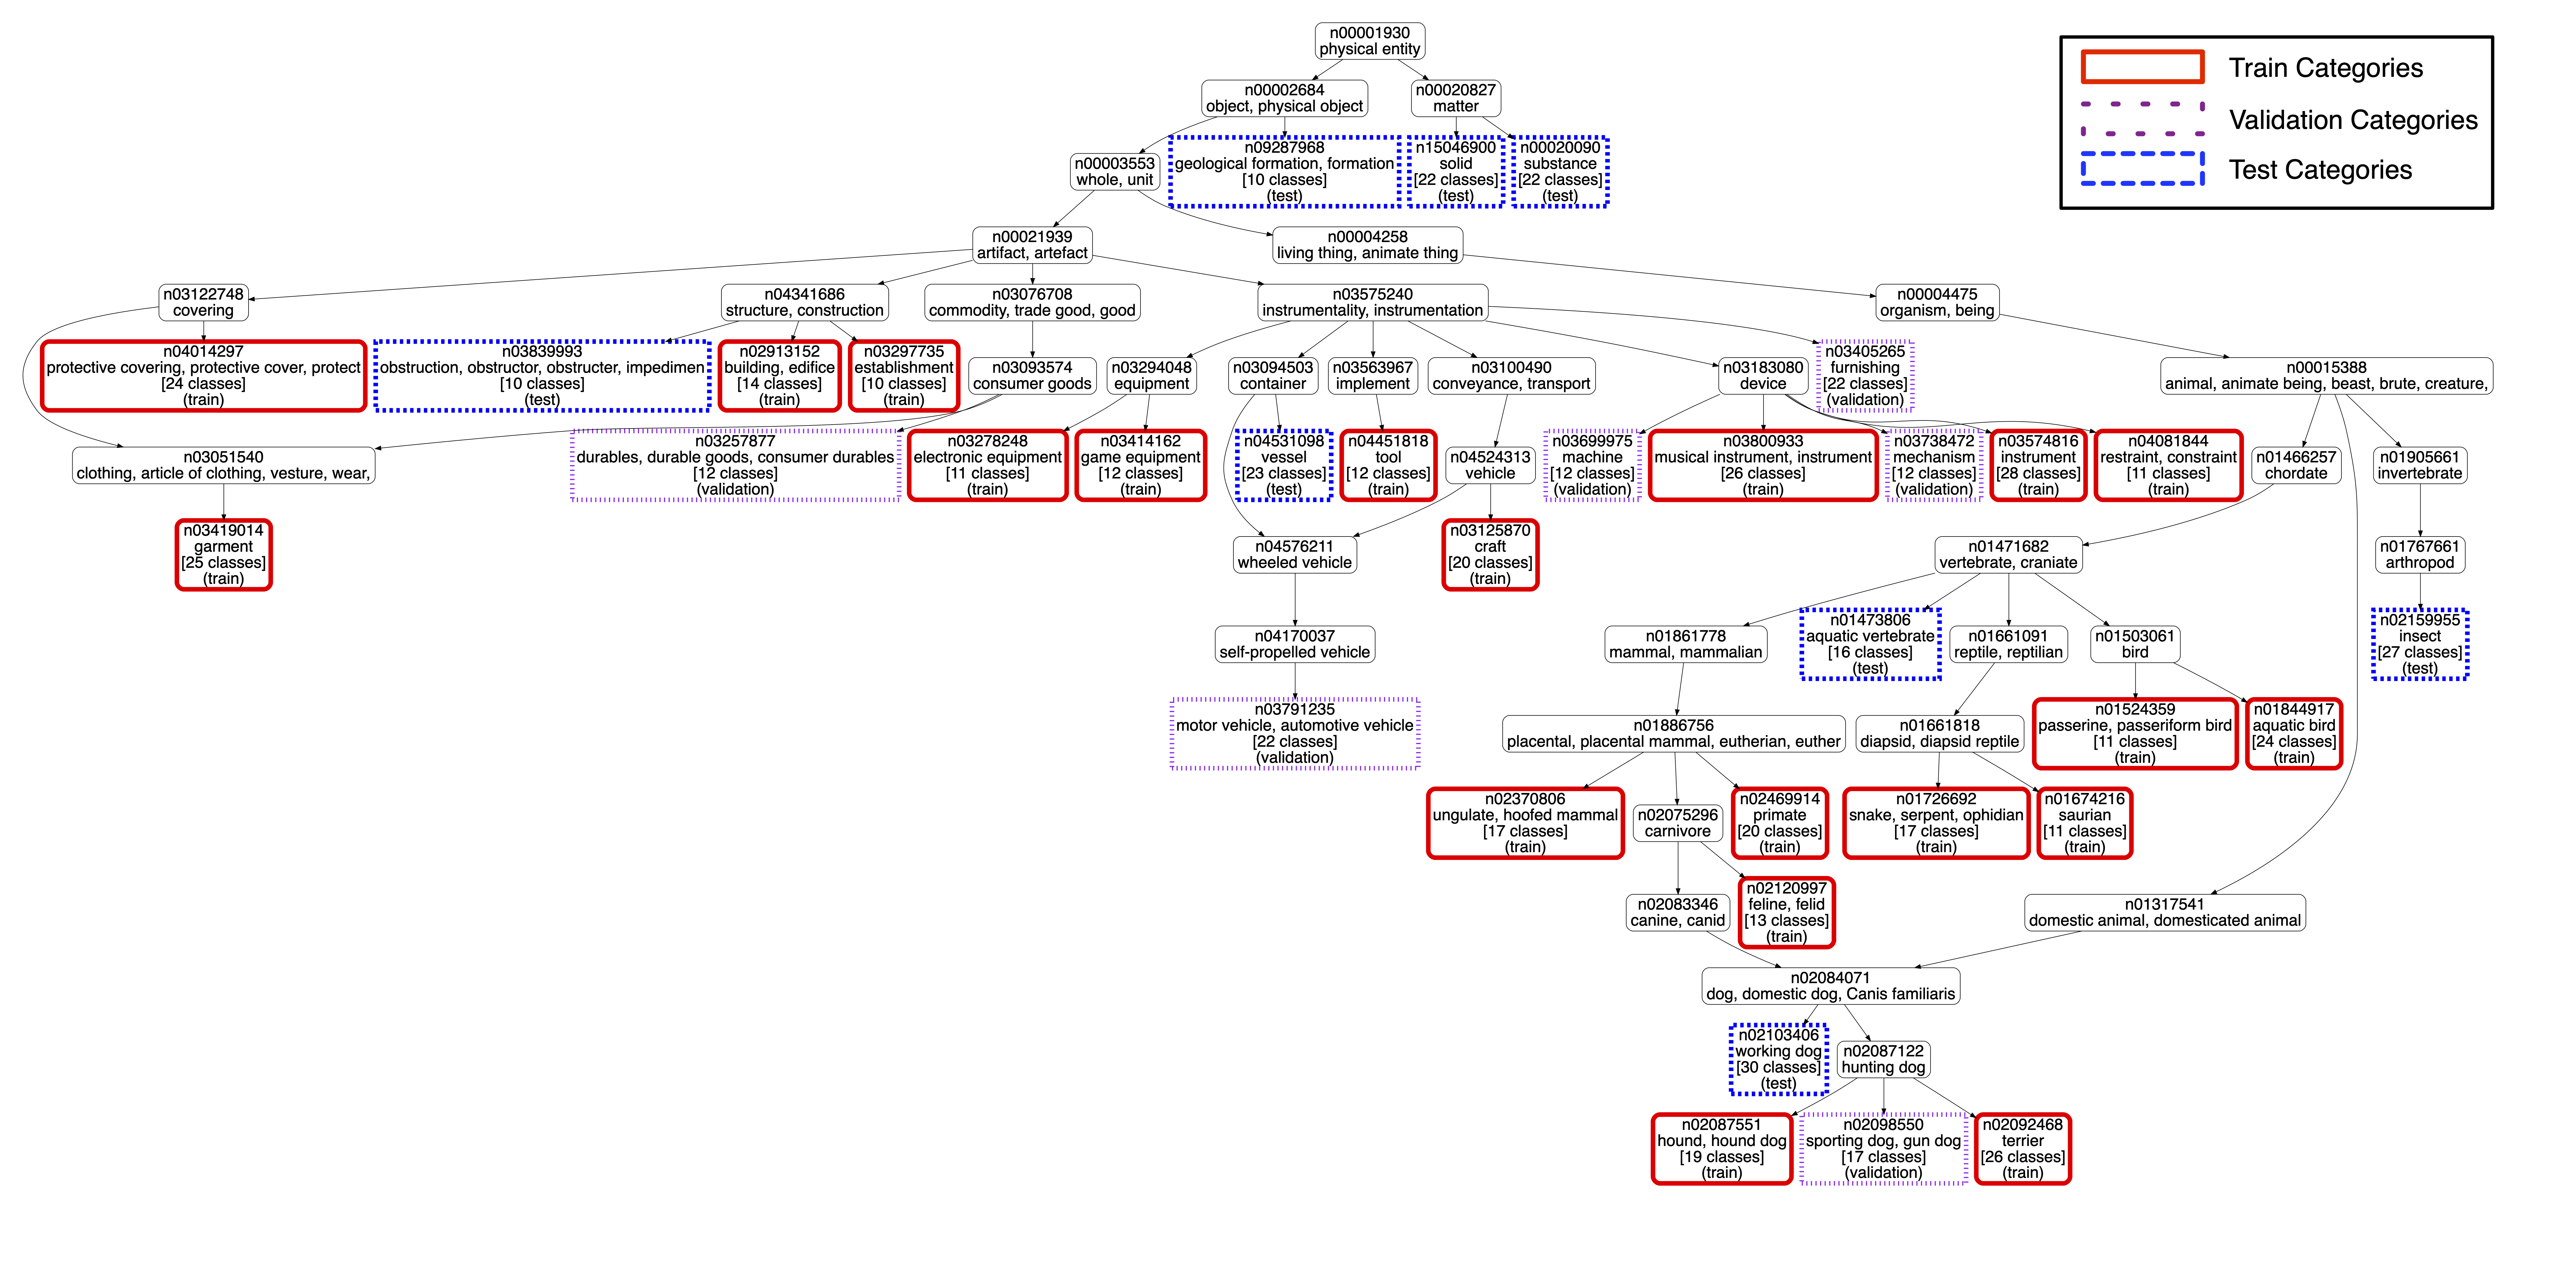
\includegraphics[width=8\textwidth]{figures/hierarchy_legend_val.png}
    \caption{Hierarchy of \textit{tiered}Imagenet categories. Training categories are highlighted in red and test categories in blue. Each category indicates the number of associated classes from ILSVRC-12. Best viewed zoomed-in on electronic version.}
    \label{fig:tiered_hierarchy}
\end{figure}
\else
\begin{sidewaysfigure}[ht]
    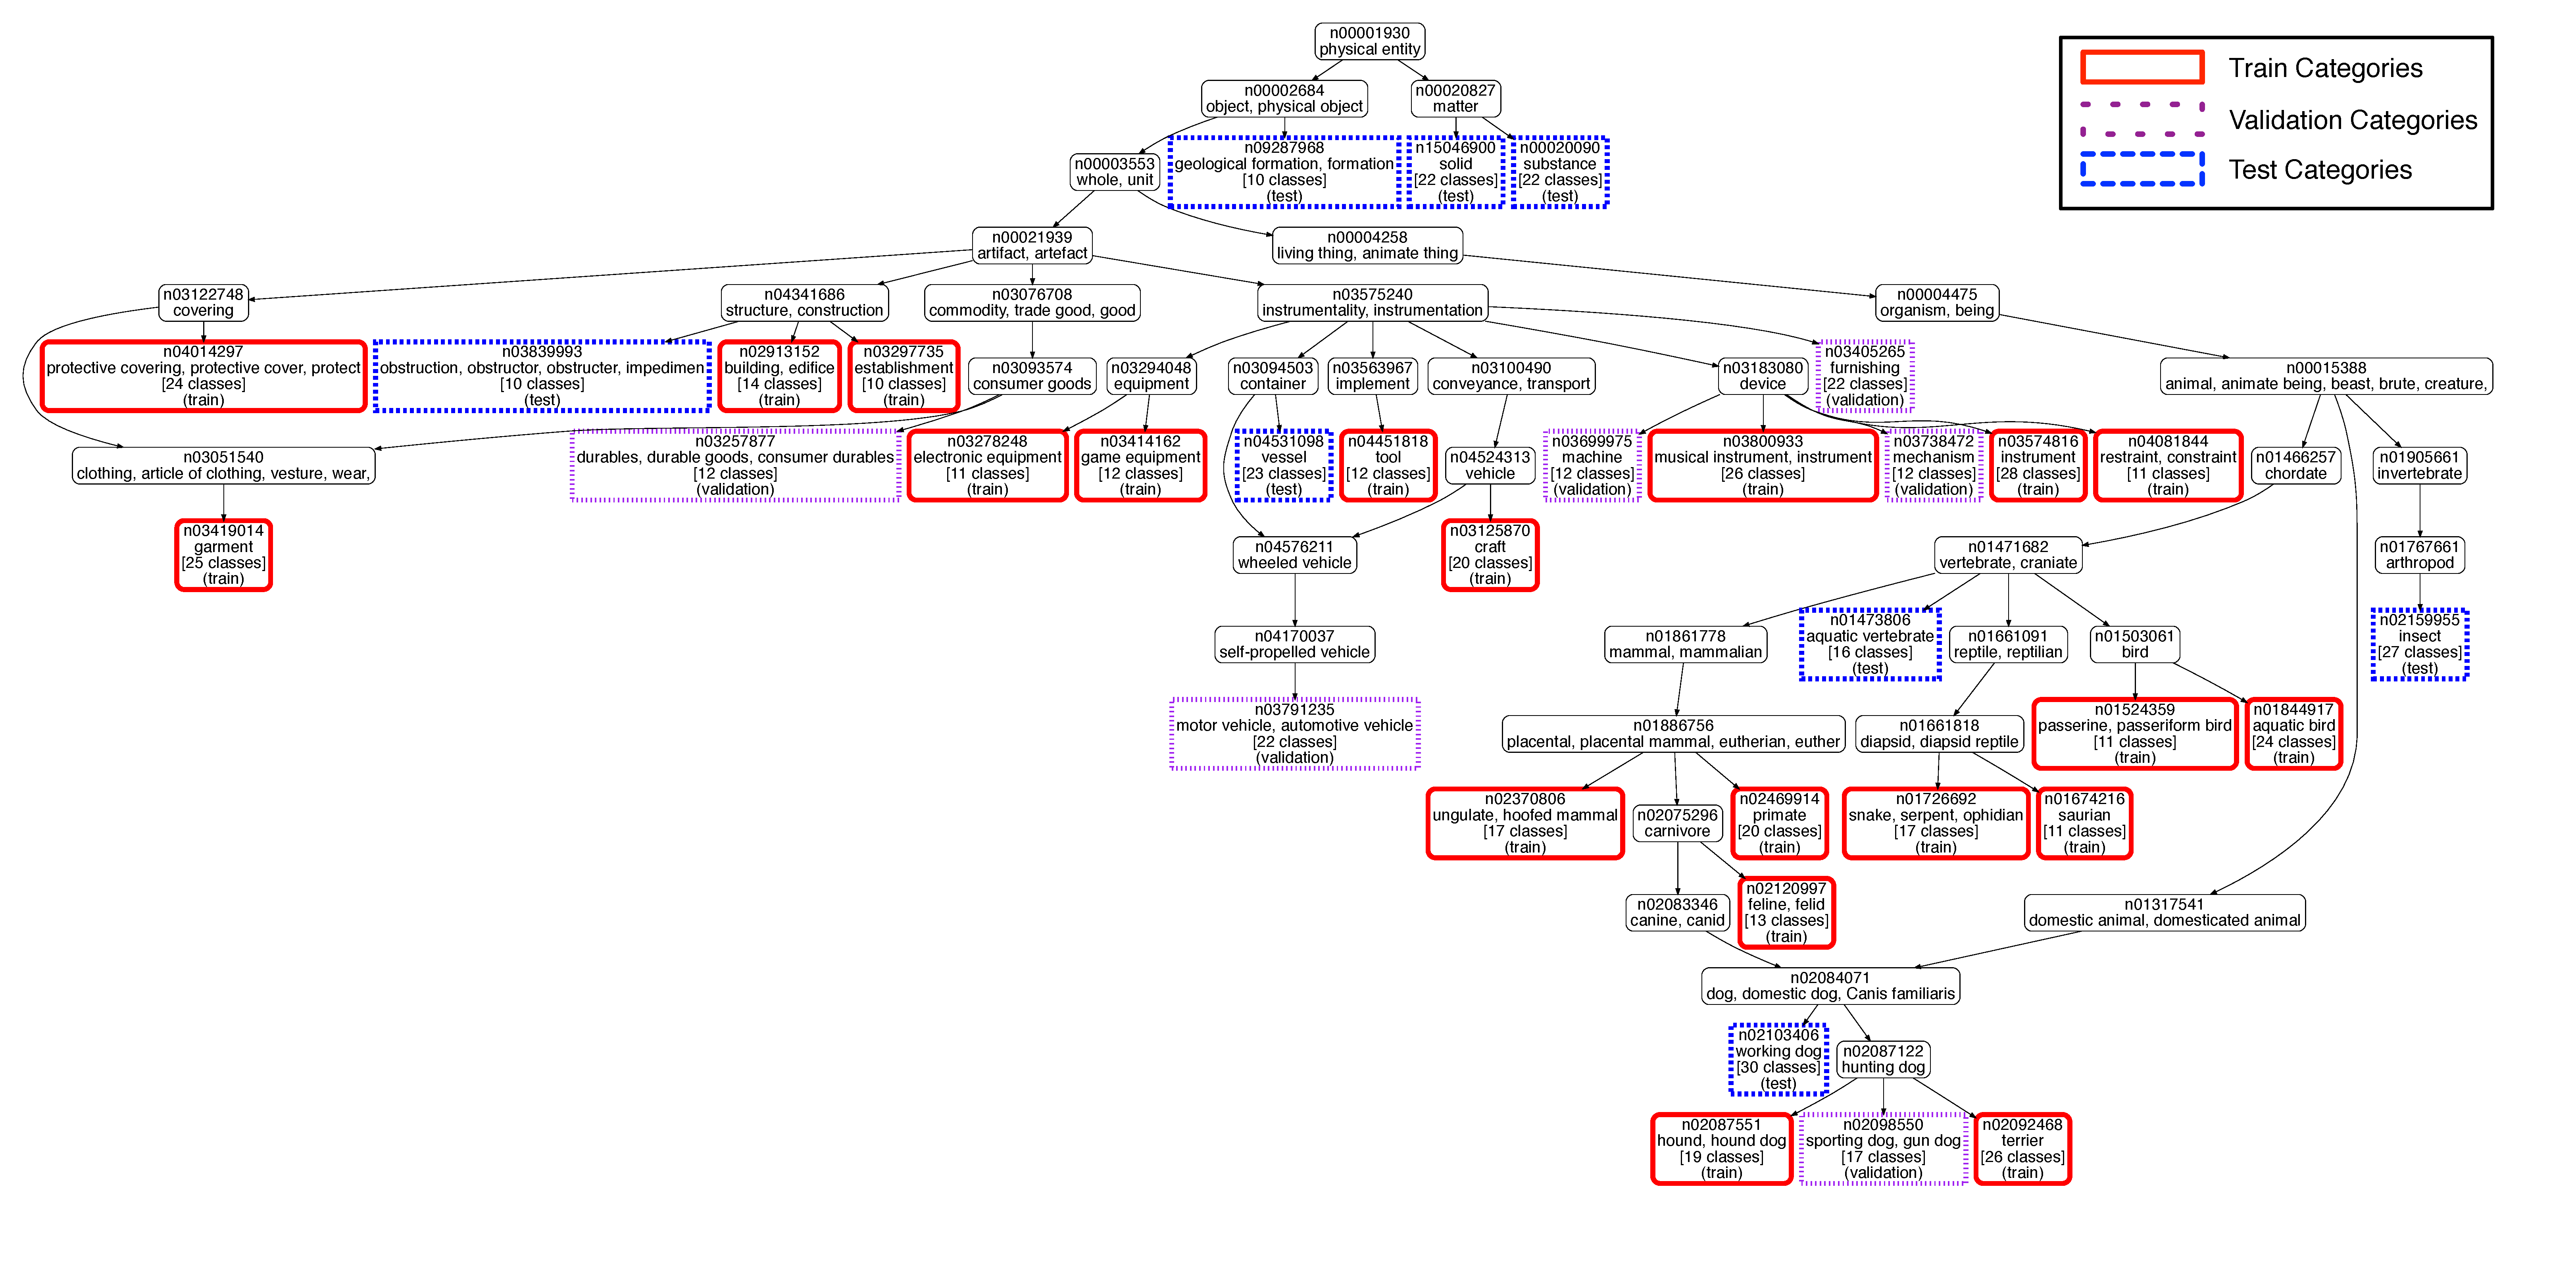
\includegraphics[width=\textwidth]{figures/hierarchy_legend_val.pdf}
    \caption{Hierarchy of \textit{tiered}Imagenet categories. Training categories are highlighted in red and test categories in blue. Each category indicates the number of associated classes from ILSVRC-12. Best viewed zoomed-in on electronic version.}
    \label{fig:tiered_hierarchy}
\end{sidewaysfigure}
\fi

\section{Extra Experimental Results}
\subsection{Few-shot classification baselines}
We provide baseline results on few-shot classification using 1-nearest neighbor and logistic
regression with either pixel inputs or CNN features. Compared with the baselines, Regular ProtoNet
performs significantly better on all three few-shot classification datasets.

\begin{table}[t]
    \centering
    \resizebox{\textwidth}{!}{
    \begin{small}
    \begin{tabular}{l|c|c|c|c|c}
                 & Omniglot            & \multicolumn{2}{c|}{\textit{mini}ImageNet}& \multicolumn{2}{c}{\textit{tiered}ImageNet}\\
    \cline{2-6}
    Models       & 1-shot              & 1-shot              & 5-shot              & 1-shot              & 5-shot               \\
    \hline
    \hline
    1-NN Pixel   & 40.39 $\pm$ 0.36    & 26.74 $\pm$ 0.48    & 31.43 $\pm$ 0.51    & 26.55 $\pm$ 0.50    & 30.79 $\pm$ 0.53     \\
    1-NN CNN rnd & 59.55 $\pm$ 0.46    & 24.03 $\pm$ 0.38    & 27.54 $\pm$ 0.42    & 25.49 $\pm$ 0.45    & 30.01 $\pm$ 0.47     \\
    1-NN CNN pre & 52.53 $\pm$ 0.51    & 32.90 $\pm$ 0.58    & 40.79 $\pm$ 0.76    & 32.76 $\pm$ 0.66    & 40.26 $\pm$ 0.67     \\
    \hline
    LR Pixel     & 49.15 $\pm$ 0.39    & 24.50 $\pm$ 0.41    & 33.33 $\pm$ 0.68    & 25.70 $\pm$ 0.46    & 36.30 $\pm$ 0.62     \\
    LR CNN rnd   & 57.80 $\pm$ 0.45    & 24.10 $\pm$ 0.50    & 28.40 $\pm$ 0.42    & 26.55 $\pm$ 0.48    & 32.51 $\pm$ 0.52     \\
    LR CNN pre   & 48.49 $\pm$ 0.47    & 30.28 $\pm$ 0.54    & 40.27 $\pm$ 0.59    & 34.52 $\pm$ 0.68    & 43.58 $\pm$ 0.72     \\
    \hline
    ProtoNet     &\tb{94.62 $\pm$ 0.09}&\tb{43.61 $\pm$ 0.27}&\tb{59.08 $\pm$ 0.22}&\tb{46.52 $\pm$ 0.32}& \tb{66.15 $\pm$ 0.34} 
    \end{tabular}
    \end{small}
    }
    \caption{Few-shot learning baseline results using labeled/unlabeled splits. Baselines either
    takes inputs directly from the pixel space or use a CNN to extract features. ``rnd'' denotes
    using a randomly initialized CNN, and ``pre'' denotes using a CNN that is pretrained for
    supervised classification for all training classes.}
    \label{tab:tieredImageNet}
\end{table}

\subsection{Number of unlabeled items}
Figure~\ref{fig:tnet_num_unlabel_text} shows test accuracy values with different number of unlabeled items during test time. Figure~\ref{fig:histo} shows our mask output value distribution of the masked soft k-means model on Omniglot. The mask values have a bi-modal distribution, corresponding to distractor and non-distractor items.
\begin{figure}
    \centering
    \iflatexml
    \includegraphics[width=6\textwidth]{figures/tnet_num_unlabel_text.png}
    \else
    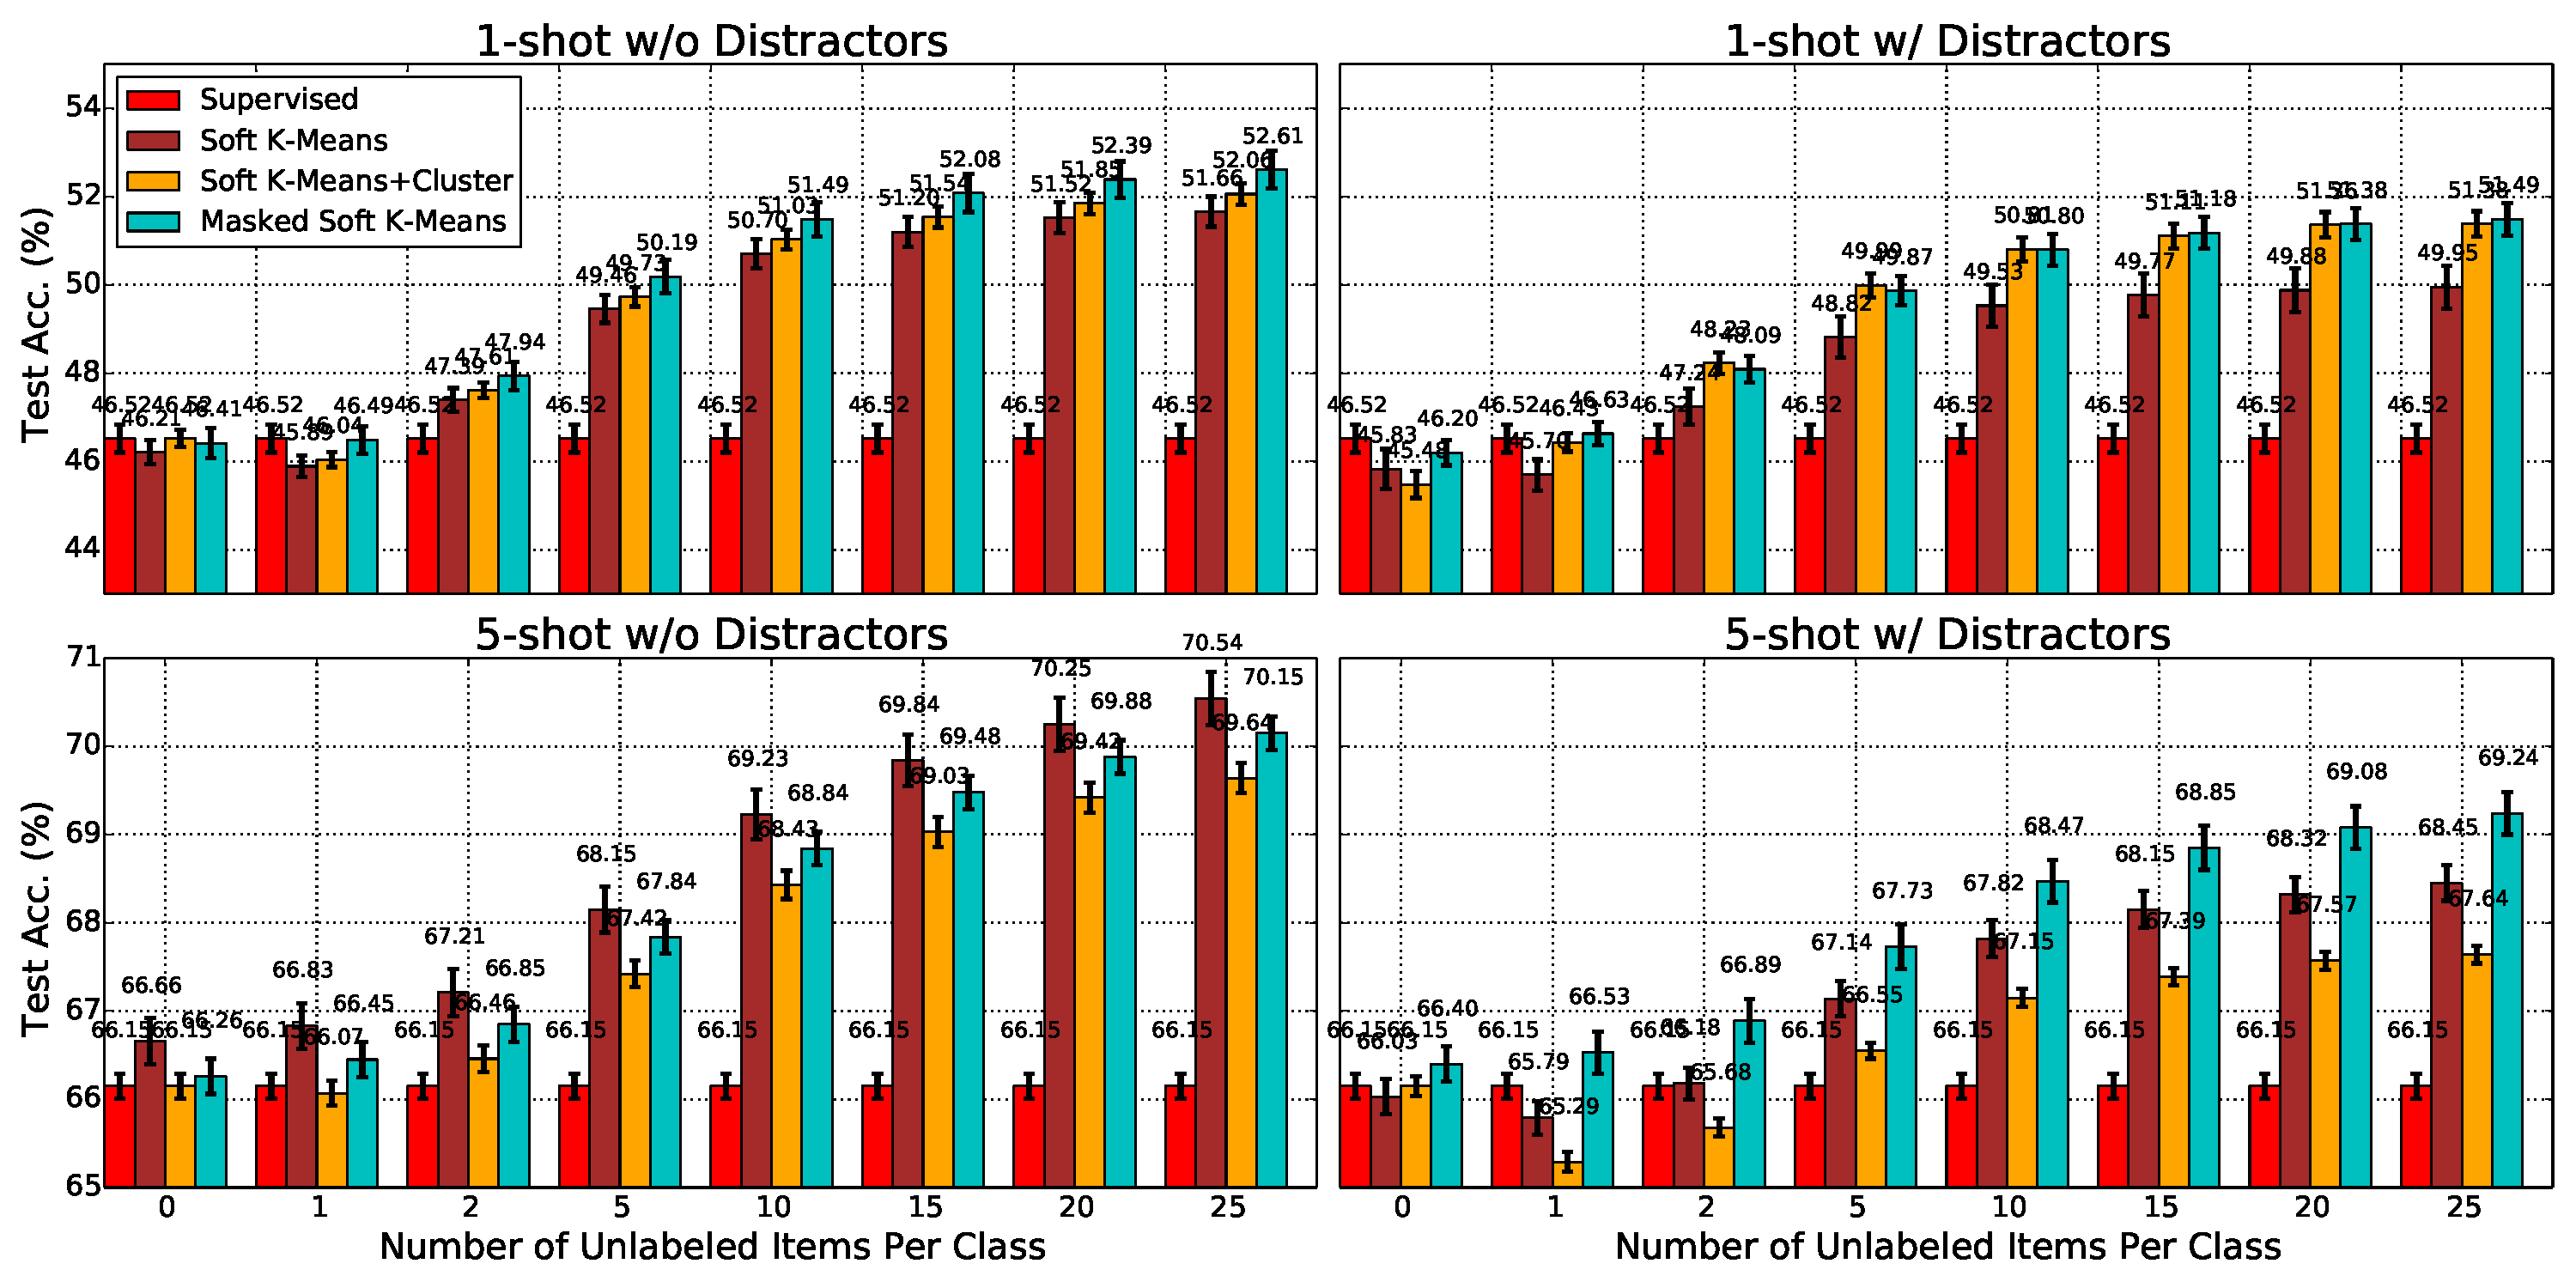
\includegraphics[width=\textwidth]{figures/tnet_num_unlabel_text.pdf}
    \fi
    \caption{Model Performance on \textit{tiered}ImageNet with different number of unlabeled items during test time. We include test accuracy numbers in this chart.}
    \label{fig:tnet_num_unlabel_text}
\end{figure}

\begin{figure}
    \centering
    \iflatexml
    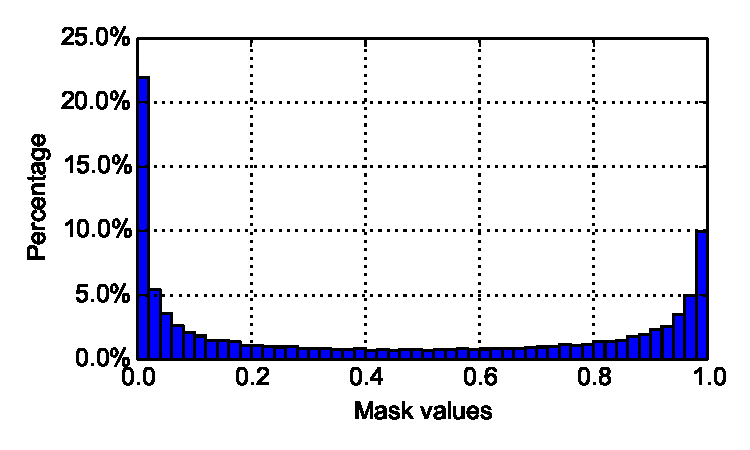
\includegraphics[width=4\textwidth]{figures/mask_histo_omniglot_refinement.pdf}
    \else
    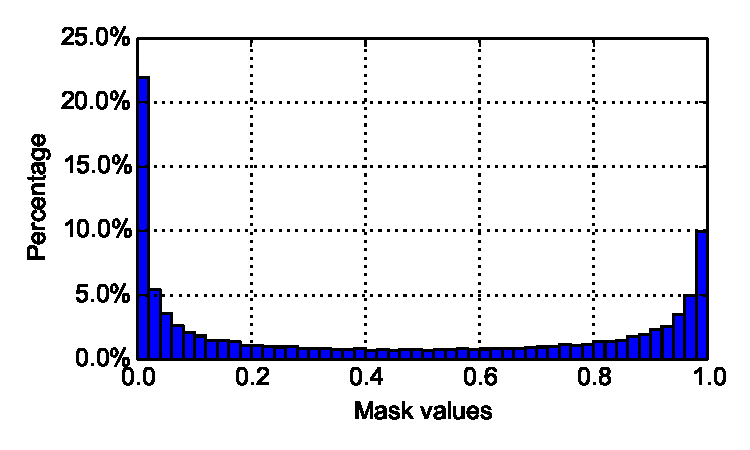
\includegraphics[width=0.7\textwidth]{figures/mask_histo_omniglot_refinement.pdf}
    \fi
    \caption{Mask values predicted by masked soft k-means on Omniglot.}
    \label{fig:histo}
\end{figure}

\section{Hyperparameter Details}
\label{sec:hyperparam}
For Omniglot, we adopted the best hyperparameter settings found for ordinary Prototypical Networks
in \cite{snell2017protonet}. In these settings, the learning rate was set to 1e-3, and cut in half
every $2$K updates starting at update 2K. We trained for a total of 20K updates. For
\textit{mini}Imagenet and \textit{tiered}ImageNet, we trained with a starting learning rate of 1e-3,
which we also decayed. We started the decay after 25K updates, and every 25K updates thereafter we
cut it in half. We trained for a total of 200K updates. We used ADAM \citep{kingma2014adam} for the
optimization of our models. For the MLP used in the Masked Soft $k$-Means model, we use a single
hidden layer with $20$ hidden units with a tanh non-linearity for all $3$ datasets. We did not tune
the hyparameters of this MLP so better performance may be attained with a more rigorous
hyperparameter search.


\end{document}
